\chapter{Software Development}
\label{chapter:software}

\begin{quote}
``The strange flavour of AI work is that people try to put together long sets of rules in strict formalisms which tell inflexible machines how to be flexible.'' \\ 
--- \textit{Douglas Hofstadter}
\end{quote}

\section{Introduction and Aims}

The primary aim of this work is the development of enhanced methods for modelling short sections of polypeptide, usually at the surface of proteins. The main use of such a protocol is as a tool in the more general process of comparative modelling. 
It is almost impossible to know \textit{a priori} whether or not a novel methodology will show promise when applied to a given real-world problem. Often the only way of verifying a given approach is the process of trial and error. It is clearly of benefit to be able to rapidly experiment with multiple different algorithms in order to pragmatically find the best solution -- as Linus Pauling once said, ``The best way to have a good idea is to have lots of ideas''. For various reasons discussed in this chapter, traditional software engineering concepts do not lend themselves well to this process; mainly because such software requires a clearly predefined implementation before development begins. 

The solution to these concerns is the creation of a molecular simulation framework, or ``toolkit'', that allows the user to experiment with new algorithms. Novel algorithms can be created by the recombination of well-established and fundamental building-blocks, without the need to constantly start from the beginning. It is therefore crucial to have an adaptable foundation and modularity is paramount. 

Mike Tyka and I felt, at the beginning of our PhDs, that such a framework was not available to us. A fruitful collaboration quickly ensued, which has ultimately resulted in the creation of a novel simulation engine, currently combining over seven man-years of development. This engine focuses on rapid algorithm development, both for ourselves and for new researchers in the future. It is now in a state to be of real use, representing a significant advance over traditional implementations.

In addition to the simulation engine, it is also important to implement facilities for the extraction and subsequent processing of data from the PDB and other experimental sources. To this end, a second framework has also been developed in parallel with  a different overall aim to that of the first. This framework lacks simulation capabilities, but is instead concerned with error-tolerant data extraction and supplies many convenient methods for subsequent processing and visualisation.  It again focuses on the primary principles of flexibility and extensibility and the current implementation is used throughout this work. Additional tools for 3D molecular visualisation and data graphing have been developed which rely upon the common underlying framework.

The aim of this chapter is threefold. Firstly current coding practices are discussed to orient the reader with respect to recent software engineering advances. These advances are used throughout the software developed for this thesis. Secondly, existing third-party simulation frameworks are discussed. Finally, the simulation and data extraction engines are discussed in turn. Initially an overview of the implementation of each framework is presented. Potential roles and typical usage of the software are then discussed. Finally the core code elements are discussed. It is not the intension here to provide a manual for any of the software; as such documentation is available in a more comprehensive form online from the group website. The development snapshot of the source code at the time of writing is included on an enclosed CD.


\section{Modern Coding Practice} 

Before discussing the specifics of the software developed for this thesis, it seems pertinent to briefly discuss modern coding standards and techniques.
It is hoped that this will illustrate how the developed code-bases  relate
to cutting-edge software development.
 
 
\subsection{Compiled Source Code}

The fundamental language of a modern computer is \emph{machine code}; essentially
a short list of basic operations that can be performed on data. Such language, to
a human, is incredibly verbose, cryptic and generally  difficult to understand. As such,
higher level languages have been developed which are human readable, but
can be \emph{compiled} into machine code. Modern compilers are well tailored
to this practice and generate highly efficient machine code from the
corresponding human readable source code. This results in what is termed an executable,
or binary, which can then be invoked on a host computer to manipulate data.

A choice of computer languages exist, all of which are best suited to different applications.
Historically, procedural languages have been extensively used throughout the academic environment.
Through experience within the software industry, a number of difficulties with this paradigm have been
found and are discussed briefly below. To address these issues, modern applications
are written under a new paradigm termed object oriented programming
(OOP). This is extensively used throughout this work and is also discussed below.  
 
\subsection{Procedural Languages}

The procedural programming paradigm is based upon the concept of top-down functional decomposition -- essentially, breaking
a problem down into a collection of procedural calls, conditional statements and primitive data arrays.
Procedural calls are also termed function calls, but should not to be confused with mathematical functions; each one performs a list of defined operations on data. After a procedural program is initiated, based on user input, a defined execution path ensues.

Common procedural languages used in the academic environment are Fortran and C, which have been around since the 1950s and 1970s respectively. As C is a more recent language
it less common in the academic environment. Both languages exhibit a minimalistic design with tightly defined language structure.\ This results in code which can be highly optimised
by the compiler and thus run in less time. This makes both languages especially suited to numerically intensive computation and scientific computing.  
Importantly, over the abilities of Fortran-77, C facilitates very powerful low-level access to computer memory.

\subsection{Object Oriented Languages}

Today, software applications are larger and more complex than ever before. The majority
of the cost of a modern software is in its maintenance --  fixing errors, modification, adding options -- often costing twice that of the
original software development. As such, it is critical that software frameworks
never ``re-invent the wheel''; meaning that overlapping functionality should be minimised and that standardised libraries, techniques and algorithms should be used wherever possible. This new emphasis on modularity and reusability fits neatly within the object oriented programming (OOP)  paradigm. 

In OOP, the conceptual currency of the language is the \emph{object}, as opposed to the procedural call. An object, put simply, is a logical grouping of data and functions which manipulate that data. Each object has a conceptually tightly-defined purpose and if designed properly can be \emph{reused}. As each of these reusable objects can be independently tested, the development process can be simplified. 
What is ultimately gained, is that programs can be developed much more quickly, with a greater likelihood of correct behaviour.


\section{Solving Difficulties in Legacy Frameworks}
\label{section:software:proceduralprobs}

It has long been realised, not only in science but in the software industry
as a whole, that classic programming techniques have some fundamental limitations.
In this section, we discuss some of the difficulties that arise from
the use of the procedural paradigm and how OOP attempts to solve some of these
problems. This is by no means intended as a comprehensive review of OOP practice,
as such literature is available in abundance, but is intended as a brief
overview for potential advantages of OOP in the scientific software environment. All the enhancements described here are used throughout this work.

\subsection{Problem 1: Global Data Scope}

The following code-snippet, listing \ref{listing:software:prob1}, shows a tiny but typical procedural application which accomplishes a given task based on user input. In this simple example all is well; the user is given just two options and the application behaves as expected, reporting the user-chosen code-path and the resultant calculated energy. This procedural paradigm, however, begins to fail as   one wants to give the user additional options and application size
increases.  

\lstset{language=CSharp}
\begin{lstlisting}[float, caption={Example procedural pseudo-code (C-like).}, label=listing:software:prob1] 
double energy; // A global variable storing the energy of the system

// A fixed-length global array of double precision floating point numbers holding atomic radii
double radius[100]; 

void setupRadii( int codePath ); // A function to fill the radius array based on the code path

// Global forcefield function calls which calculate the energy of the system using
// the global radius array, and stores the result in the global variable `energy'.
void forcefieldA(); // A forcefield calculation, coded by person A
void forcefieldB(); // A forcefield calculation, coded by person B

// Our program begins with a call to the function main()
void main(int pathID)
{
        setupRadii( pathID ); // Setup the radii dependent on the user specified code path

        if( pathID == 1 ) { forcefieldA(); } // Run forcefieldA
        else if( pathID == 2 ) { forcefieldB(); } // Run forcefieldB
        else 
        {
            printf{"Please enter either option 1 or 2. You entered %d",pathID);
            return; // Exit early without printing the energy
        }

        // Report the execution path and calculated energy to the user
        printf("Mode %d yields an energy of %f kcal/mol", pathID, energy );

        return; // We completed successfully
}

\end{lstlisting}

The main concern in this implementation, is that both forcefield() calls use the same global data array to store radii. What if each forcefield calculation requires different atomic radii? An easy solution might be to simply create two independent and persistent global arrays of radii, radiusA and radiusB. However, this practise quickly becomes impractical as the total number of forcefield functions increases. As all data is global, it can be modified by any function at any time, which makes tracking down errors intrinsically difficult. Each array must be separately maintained, typographical errors can result in the modification of the wrong data array \emph{without warning} and many of the arrays will be completely redundant for multiple code-paths.
Naive array duplication is clearly not a good solution.


Instead, as in listing \ref{listing:software:prob1}, we could call a setup() function prior to each forcefield() call, with each function reliant on the same global data array. Each function then has specific requirements about when and where it can be called and what \emph{must} be called beforehand. Critically, it is common for this practise to result in incompatibilities, especially when different code-paths are implemented by different people. In addition,
when a user requests an unusual selection of application parameters, strange and undefined effects can occur. The application itself must therefore be carefully designed and documented; but this process \emph{requires} specialist knowledge of the entire code-base, not just for the developer, but in the worst cases also the \emph{user}.

Even if one is very careful, with multiple developers, this process rapidly becomes unmanageable and so classical procedural applications are usually small and limited to a single well-defined task. This, however, results in applications with overlapping functionality. For these separate applications to interact, they must communicate via common-format input and output files, coordinated by shell scripts; a process that is again  messy and error-prone.  Many small scientific applications actually share a good deal of common ground, such as how to read structural data from a file, but each one must be maintained and upgraded separately when new features or performance enhancements are created.


\subsection{Solution 1: Class-based Architecture}

 We have already mentioned that in OOP, the fundamental building-block of an application is
the \emph{object}. Put simply, an \emph{object} is a humanised grouping of data. Each object is self-contained and combines both data and functions into one neat package. The technical terminology is that an \emph{object} is as an instance of a \emph{class} -- a \emph{class}
being the blueprint for a given type of \emph{object}. The rules for the interrelationships between various objects are subsequently enforced by the compiler. 

\subsubsection{Class Scope}

Procedural applications essentially only have global and local \emph{scope} -- scope simply defines the lifetime of data. Global
scope data persists from initiation to termination of the application as a whole and can be changed at any time by any function. Local scope data,
defined at the start of a function call, expires  when the function terminates.
OOP\ languages extend this by adding class scope, where the data is only accessible via the  object to which it belongs and exists for the lifetime of that object.

Not all persistent data and associated functions need to be accessed globally and hence their interface should be tightly defined;
only a function that needs access to data should be granted such access. Importantly, class scope  data and functions can be made \emph{private}, which means that they can only be accessed from within the object itself.  This greatly reduces software development time and maintenance cost because there are fewer potential sources of logical errors -- the compiler will catch data-access logic errors at compile-time, preventing their propagation to run-time.

\subsubsection{An Example}

Let us revisit the example put forward in listing \ref{listing:software:prob1}.
In the new version, shown in listing \ref{listing:software:sol1}, we introduce
the ForcefieldA class, which conceptually embodies everything to do with  implementation-A of a forcefield as a single self-contained unit. Importantly,  the radius array and setupRadii() call are class-scope and made private; meaning that they can only be used by functions belonging to ForcefieldA. By contrast, print() and evaluate() represent the \emph{public interface} and can be called at any time, but only by client functions that possess a reference to a ForcefieldA object. 

\lstset{language=CSharp}
\begin{lstlisting}[float, caption={Example  OOP pseudo-code (C++).}, label=listing:software:sol1] 
// The *abstract* concept of a forcefield is embodied by a class structure
// Implementation A
class ForcefieldA
{
public:
        // The class constructor is called automatically when an instance of ForcefieldA is made
        ForcefieldA()        
        {
            setupRadii();    // the object configures itself when it is created
        }

        double evaluate();   // Returns the current energy
        void   print();      // Prints the current energy, calling 'evaluate' internally
private:
        void   setupRadii(); // Fill the radius array based on the code path
        double radius[100];  // Private radius array belonging to this instance
};

// Implementation B
class ForcefieldB
{
public:
        // The class constructor is called automatically when an instance of ForcefieldB is made
        ForcefieldB()
        {
            setupRadii();    // the object configures itself when it is created
        }
        double evaluate();   // returns the current energy
        void   print();      // prints the current energy, calling 'evaluate' internally
private:
        void   setupRadii(); // Fill the radius array based on the code path
        double radius[100];  // Private radius array belonging to this instance
};

// Our program begins with a call to the function main()
void main(int pathID)
{
        if( pathID == 1 ) 
        { 
                ForcefieldA ff; // Here we create an instance of ForcefieldA
                ff.print();     // and ask it to print its energy
        }
        else if( pathID == 2 ) 
        { 
                ForcefieldB ff; // Here we create an instance of ForcefieldB
                ff.print();     // and ask it to print its energy
        }
        else 
        {
            printf{"Please enter either option 1 or 2. You entered %d",pathID);
            return; // Exit early without printing the energy
        }
        return; // We completed successfully
}

\end{lstlisting}

Therefore, by using objects, we solve problem 1. Firstly there is predominantly no longer any need for global data.
Each data element is tightly associated with its parent object, and can \emph{only}
be accessed through that object.
Secondly, we no longer have the difficulty that ForcefieldA can be, in any way, influenced
by the actions ForcefieldB. Finally, there is no waste, because a class instance is only created in memory when it is needed.
 
\subsubsection{Additional Benefits}
 
Importantly, as
each class tightly defines only its public interface, classes also provide intrinsic
modularity in the code. This means that the internal implementation of a given feature can be changed
at a later date, usually to increase efficiency or correct errors. As long as the interface itself doesn't change,  no other
code which depends on it will be broken. This means that testing is
confined to a single class and reduces maintenance time. Finally, after a
set of complementary class interfaces are agreed, a single developer can work on the implementation
of each interface, simplifying and accelerating the development process.   






\subsection{Problem 2: Code Duplication and Stagnation}

In procedural programming, tasks such as sorting a list of atomic Cartesian coordinates are usually performed by a single specialised function which looks at independent
x, y and z arrays. The same underlying algorithm
however may also be used elsewhere in the code that simply sorts a list of integers
or floating point numbers. Critically, each \emph{requires} a separate function, all of which must be separately maintained
but in essence implement the same underlying algorithm but for different data structures. What is needed is a way of allowing
a single copy of the algorithm to work on multiple different but analogous data types. 



\subsection{Solution 2A: Class Inheritance}
\label{section:software:inheritance}

We have already discussed how conceptual groups of data and functions can be combined within a single object. Many of these objects actually share a good deal of logic. As has been discussed, code duplication should be avoided at all costs, to
decrease the maintenance burden for a given application.  A mechanism for sharing common functionality between objects is a technique
called \emph{inheritance}, illustrated in listing \ref{listing:software:inheritance}.

\lstset{language=CSharp}
\begin{lstlisting}[float, caption={Class inheritance.}, label=listing:software:inheritance] 
class Position // A class describing a Cartesian position
{
public:
    double x;
    double y;
    double z;
    
    void moveToOrigin();                // Move to 0,0,0
    void moveTo( Position& newPos );    // Move to a position in Cartesian space
    void moveBy( Position& newPos );    // Displace by a Cartesian vector
    void rotate( RotationMatrix& rot ); // Rotate in space using this matrix
    void print();                       // Print the current location
}

class Atom : public Position // Derive Atom from Position
{
public:
   int index;
   std::string name;
   double radius;
}

// A function which does something to a position in space
void manipulatePosition( Position& pos );

void main()
{
    Atom a;                // Create an atom
    a.x += 12.0;           // Add 12 to the X coordinate of Atom a
    a.moveToOrigin();      // Move the atom to the origin
    manipulatePosition(a); // Perfectly legal, as an atom IS also a position
}

\end{lstlisting}

Take, for example, an atom. In a typical implementation of a molecular simulation, an atom is essentially
a position in Cartesian space with additional properties, such as a  radius, numeric index or name. For geometric manipulation, the kind of things one wants to perform on an atom are essentially the same as for any other position in space. What is needed is a way of giving an atom the same properties
as a position without duplicating the underlying code. To do this we \emph{derive} \textsl{Atom}
from \textsl{Position}, and subsequently \textsl{Atom} gains all the properties of a Cartesian position; consequently, \textsl{Position} is the \emph{base class} of \textsl{Atom}.

This has a number of important implications. Firstly, any function that can
work on a \textsl{Position}, such as sorting, can now also work on an \textsl{Atom}. This requires
no code duplication. Secondly, when we upgrade Position with new features or a
performance enhancement, \textsl{Atom} implicitly gains these new abilities.  Finally,
and perhaps most importantly, such abstractions are very intuitive to the user -- one expects to be able to move an \textsl{Atom} in space and therefore treat
it as a \textsl{Position}.

\subsection{Solution 2B: Template Meta-Programming}
\label{section:software:templates}

A recent and extremely useful language development is template meta-programming.
Meta-programming is essentially code which creates further tailored code on demand. Say for example we need a function that adds together all the
elements in an array and we have integer, floating-point and position arrays.
In standard procedural and indeed more basic OOP languages, one would have to create three
specialised functions which essentially do the same thing, but on different
data types. Listing \ref{listing:software:template} shows how templates allow the programmer to tell the compiler to \emph{automatically}
create these functions.  This means that common algorithms need only be coded and maintained once and can be re-used between multiple problems. 

\lstset{language=C++}
\begin{lstlisting}[float, caption={Template meta-programming.}, label=listing:software:template] 
// The traditional method; copy and paste the algorithm.
double   sumArray( double* data,   int count ); 
int      sumArray( int* data,      int count );
Position sumArray( Position* data, int count );

// The template form, whereby T is essentially a wildcard. The compiler automatically duplicates
// the function body and replaces T with each type that is actually used within the application.
// The end result is that the three functions are defined by just one general function, 
// In this case, 1/3 of the effort is thus required.
<template T>
T sumArray( T* data, int count )
{
   T sum = 0;
   for( int i = 0; i < count; i++ ) // iterate over all data
       sum += data[i]; // add data element `i' and sum, storing the result in sum
       
   return sum;
}
\end{lstlisting}

It should be noted that the same effect may be obtained with weakly-typed and dynamic languages such as Perl and Python respectively, whereby interpretation of a given code line
occurs at runtime rather
than at compile time. It is worth noting, however, that such practice comes
with an associated performance penalty and so is less suitable for use with high performance
scientific code. An additional problem with these languages is that, as machine code is
generated at runtime, some logic checks cannot be performed by the compiler.
This means that some types of code error can be retained until further along the development path. 







\subsection{Problem 3: Static Memory Allocation}

Fortran-77 does not allow dynamic memory allocation, requiring that the
size of all arrays be pre-defined at compile time. The programmer decides
that the largest molecular system that will be imported will contain 10,000
atoms and sets this limit. As is usual, some time later someone has a more powerful
computer and wants to simulate a larger system -- they can't. If the application
source code is still available and has been well designed, these limits
can easily be increased and the application recompiled. However, this results in multiple
versions of the application, where the new version will no longer execute on older computers. In addition, not all of the static arrays will be used to capacity,
resulting in significant waste for the original smaller molecular systems and requires higher specification hardware to facilitate
execution.
Furthermore, the addressing of larger memory ranges inevitable has an associated performance penalty, as larger data arrays are less likely to remain within the limited CPU level 1 and level 2 caches.

\subsection{Solution 3A: Dynamic Memory Allocation}

Compared to Fortran-77, newer procedural languages like C are more powerful as they allow dynamic memory allocation. Thus, the issue is not directly with procedural languages  \mbox{\textit{per se}}, but relates more to the limits imposed by the use of legacy languages and compilers. In listing \ref{listing:software:memory} we show how memory could dynamically be created in C to hold a set of $n$ Cartesian coordinates.
The principle advantage of this is that, at any given point, only the memory that is needed has been allocated. The disadvantage is that this memory then needs to be \emph{managed} by the programmer, a task which is non-trivial and error prone.
\lstset{language=C++}
\begin{lstlisting}[float, caption={Static versus dynamic memory allocation.}, label=listing:software:memory] 
// The legacy way - a static, fixed-length structure of arrays
#define SYSTEM_SIZE 100;
double x[SYSTEM_SIZE];
double y[SYSTEM_SIZE];
double z[SYSTEM_SIZE];

// The C way - a dynamic array of structures
typedef struct pos_data
{
    double x;
    double y;
    double z;
} Position;

Position* makePositions( int n )
{
    // Allocate new memory to contain the new atoms
    // and return the address of the allocated memory.
    // This memory *must* be freed later...
    Position* atoms = (Position*) malloc( sizeof(Position) * n ); 
    return atoms;
}
\end{lstlisting}



\subsection{Solution 3B: Container Classes}

Modern OOP takes dynamic memory allocation a step further by making
it more user friendly, powerful and less error-prone with the advent of container
classes; illustrated in listing \ref{listing:software:containerclass}.
These are used frequently in OOP programs when the programmer requires \emph{dynamic} arrays of a given type of object. There 
are different types of container for different purposes, including lists, stacks (first
in, first out) and queues (first in, last out).
Each container class utilises templates (section \ref{section:software:templates}) and can, therefore, be created for any object type. 
All containers classes automatically manage their internal memory and come with built-in functionalities, allowing
them to be dynamic -- they can change size during program flow, having elements deleted or maybe duplicated.

\lstset{language=C++}
\begin{lstlisting}[float, caption={The power of container classes.}, label=listing:software:containerclass] 
void print( std::vector<double>& data )
{
    printf("Data: "); // Print a header
    for( size_t i = 0; i < data.size(); i++ ) // data knows its own array length via size()
    {
        printf("%3.1f, ",data[i]); // print data element i to 1 decimal place
    }
    printf("\n"); // New line
}

void main()
{
    std::vector<double> myData; // A container for double precision floating point numbers
    myData.push_back(4.0);
    myData.push_back(9.0); // Add some data to the container
    myData.push_back(1.0);
 
    std::vector<double> myDataB; // Create a second container
    myDataB = myData; // Copy all the data from myData into myDataB

    print( myDataB ); // Print the copied data
    myDataB.erase(myDataB.begin()+1); // Erase the second container element (element 1)
    print( myDataB ); // Print the data following manipulation
    myDataB.insert( myDataB.begin(), 8.3 ); // Insert 8.3 at the beginning
    print( myDataB ); // Prove its worked
    print( myData ); // Show the original array remains unchanged

}

// Application Output:
// Data: 4.0, 9.0, 1.0, 
// Data: 4.0, 1.0, 
// Data: 8.3, 4.0, 1.0, 
// Data: 4.0, 9.0, 1.0,
\end{lstlisting}

All these highly optimised and well planned container classes are provided as standard with all modern OOP languages. In \CPP\ they are provided within the standard template library (STL). Importantly, every programmer will be instantly familiar with these classes, reducing  the learning-curve for any new developers. 

A second major advantage of container classes is the built-in provision for common every-day algorithms, such as sorting, illustrated in listing \ref{listing:software:sort}. In algorithms like sorting, the bulk of the logic is constant no matter what data is being operated on.  Traditionally, each data type required its own function with duplication of the underlying algorithm. In the example, std::sort() is provided by the STL; the only logic that is missing is exactly what makes a \textgreater\ b. The programmer provides this in what is called a \emph{predicate} -- in the context of sorting, quite simply a function that returns true if $a>b$. This vastly reduces code duplication and means that any data can be sorted by any criteria with a trivial amount of new code.\   
 

\lstset{language=C++}
\begin{lstlisting}[float, caption={Sorting.}, label=listing:software:sort] 
// Legacy!
void sortAtoms(); // Single purpose function
void sortAtoms( Position* p, int count ); // Function to sort ANY position array

// Modern -- separate the sort algorithm from the element comparison
bool testByXCoordinate( Position& a, Position& b ) // returns true if a > b
{
   // Sort based upon the X coordinate alone
   return a.x > b.x;
}
void sortAtoms(std::vector<Position>& pos )
{
    // Sort position vector via a predicate.
    std::sort( pos.begin(), pos.end(), testByXCoordinate );
}
\end{lstlisting}

As the standard container classes come with such a wealth of advantages and are both heavily-optimised and error-tested, they should be used at the core of all new applications based upon the OOP\ paradigm.











\subsection{Problem 4: Managing Program Flow}
\label{section:software:prob4progflow}

Listing \ref{listing:software:prob1} can be further used to illustrate an issue with
the chosen user interface. What if we want to execute both forcefieldA() and forcefieldB() because they describe different but complementary energetic aspects? In this simple case, a new code path must be created which calls both in turn and sums their results. The difficulty with this is when an application has been in development for a decade, it is likely to have  hundreds of different possible forcefield calls, the combinatorial management of which is likely to be very difficult.

Most scientific applications are controlled by the user via the
command line, whereby the executable is started with a series of arguments
which affect program flow. The difficulty with this model is that a user
interface for each implemented
code feature must be explicitly defined; usually by some sort of alpha-numerical
flag read from the command line or a file.
Each of these must be separately maintained and documented, but also means
that a significant amount of code is dedicated to reading and checking
these flags before execution begins.

In order to facilitate greater flexibility of execution, the creators of some well established applications such as the \amber\ and \charmm\ molecular
mechanics frameworks, have even implemented their own internal scripting languages. These, whilst
very useful, are not as powerful as a full blown programming language, allowing
only simple features like incrementation of counters, conditional statements
and the notoriously error-prone goto statement. An example of a \charmm\ script for a simple energy minimisation is shown in listing \ref{listing:software:charmm}.

\lstset{language=charmm}
\begin{lstlisting}[float, caption={Example \charmm\ script to perform an
energy minimisation, adapted from official \charmm\ documentation. The standard use of highly abbreviated commands is detrimental to the user experience; for example ``CTOFnb'' means nothing to the user without searching though complementary documentation.}, label=listing:software:charmm] 
! Read in Topology and  Parameter files
open unit 1 card read name top_all22_prot.inp 
read RTF card unit 1
close unit 1

open unit 1 card read name par_all22_prot.inp 
read PARA card unit 1
close unit 1

! Read sequence from the PDB coordinate file
open unit 1 card read name myprotein.pdb 
read sequ pdb unit 1 
close unit 1

! now generate the PSF and also the IC table (SETU keyword)
generate prot setu

! build in hydrogens if using a crystal structure
hbuild sele all end

! build in missing coordinates using values in
! the parameter set
ic fill
ic para
ic build

! non bonded interaction
NBONd  CUTNb  15.0  CTONnb  14.0  CTOFnb  14.5  SWITch  VSWItch CDIElectric EPSilon  1.0

! minimise structure
energy
mini sd nsteps 500 nprint 50
energy

stop
\end{lstlisting}



If multiple simulations are required to be integrated, it is common for these
to be managed by crude customised shell scripts. These often use error-prone
calls, with limited sanity-checks, to parse data from the output files of one application and from it somehow create an input file for the next application. 




\subsection{Solution 4: Integrated Scripting}
\label{section:software:integratedscripting}

A fairly recent innovation, to aid in the export of the features in a software framework to the user, is the integration of an existing independently-developed scripting engine. These languages, such as Python and TCL are incredibly powerful languages
in their own right. By presenting entire  classes from an underlying code-base directly to the user,
robust and easy-to-develop applications can  be written quickly. This removes all
need for explicit command line flags and associated setup functions, with the caveat that underlying
code-base is required to be very well designed to be intelligible to the end-user. Such a system is used in this work, and is discussed in more detail in section \ref{section:software:pd} 










\section{The Future of Algorithm Design}
Moore's Law\cite{COMP:Moore65} is the empirical observation first coined in 1965, stating that the number of transistors on a basic cost integrated circuit boards roughly doubles every 18-24 months. It is assumed that the number of transistors correlates with chip complexity and therefore the number of floating point operations per second (FLOPS)  for a given processor. This law has held true from 1965 until the present day, however in terms of single processor cores, Moore's Law has begun to fail. Due to the physical limitations of the electrical properties of silicone, making smaller transistors in the future will not
be possible. In order to maintain the same rate of performance increase CPU manufacturers are now releasing multi-core processors; a trend that is likely to continue for the foreseeable future. 

In the light of this transition toward multi-core architectures, within the high performance computation (HPC) community,  several prominent spokespeople\footnote{Dr. John Gustafson, ClearSpeed Technology Ltd.} have begun to raise certain issues over current algorithm design and choice of implementation. New software implementations  \emph{must} take full advantage of parallel processing techniques in order to remain competitive in performance on the latest architectures. This involves utilising parallel processing application programmers interfaces (APIs) such as OpenMP, MPI and the new
Threading Building Blocks from Intel.\ These can also be used in combination with new hardware technologies such as dedicated co-processor boards now hosted in several HPC institutions, including Blue Crystal at the University of Bristol.

A second important issue is that within current architectures a processor now takes hundreds of times longer to read a number from main memory than it does to perform arithmetic on it with fifteen-digit accuracy. Reading data from a hard drive takes orders of magnitude more time again. This intrinsically means that methods using large-scale pre-calculated
databases waste available resources as the CPU lays dormant waiting for IO access. With that in mind, high-detail all-atom calculations are becoming more computationally feasible for use as evaluators in protein structure prediction -- such calculations require comparatively little data access,
but require \emph{significant} processing power.


\section{Competing Simulation Packages}

When developing any application it is important to be aware of the competition: its strengths and weaknesses and where improvements could be  made. The following section details the most important and widespread simulation frameworks currently available.

\subsection{The Sleeping Giants}

\amber\cite{FORCEFIELD:AMBER,COMPCHEM:Pon2003} and \charmm\cite{FORCEFIELD:CHARMM} are very large and well established simulation packages written in Fortran-77.
Each package is available to academics for a small fee.
 Both have been developed by large teams of researchers over many years, originating from the archetypal molecular mechanics forcefield developments which go by the same names.
They are still under rigourous development, but are based upon the  ageing procedural paradigm.  
Notoriously inflexible, partly due to procedural code limitations discussed in section \ref{section:software:proceduralprobs}, they are difficult to
extend to provide new functionality.

In addition to the main distributions, additional code-patches exist, each of which have been developed by other individuals or groups for a given purpose. These can be logic tweaks to allow an unusual experiment or extend whole new features. Patches like this are reasonable temporary solutions, but are intrinsically hard to combine as they often conflict with each other. Eventually, some patches are integrated into the main distributions.


\subsection{More Recent Packages}

\tinker\cite{COMPCHEM:TINKER} is a free package, again written in Fortran and intended for experimentation
with new methods. It is more flexible than both \amber\ and \charmm\, but
still within the limits of Fortran. \tinker\ supports a large number of \forcefields\ and methods. There is, however, a significant amount of code duplication, mainly due to the lack of inheritance as described in section \ref{section:software:inheritance}.
\tinker\ is comprised of comparably very slow code as development has disproportionably favoured code features over performance. 

\modeller\cite{METHOD:MODELLER} is a more specialised package designed to produce comparative
protein models. Many features are built into \modeller, including\   single and multiple
sequence and
structural alignment, energetic evaluation and structure optimisation by the
satisfaction of spatial
restraints. As such, it is an excellent tool for its purpose, but lacks
more general simulation features in other packages.
\modeller\ is written in Fortran-90, but has been augmented with an explicitly defined Python-based front-end to provide scripting support.


\gromacs\cite{COMPCHEM:GROMACS} is written in C and pure Assembler (essentially machine code). Assembly language is used for core functions within the package and reflects
the developers desire for ultra-optimisation of their code-base. These inner loops
make use of all manner of the latest commonly available hardware extensions
such as SSE (Streaming Single Instruction Multiple Data Extensions). Whilst hand-written
 machine code can yield a very significant reduction in execution time, it also means that the code
is less general and much more difficult to maintain, sacrificing both flexibility and extensibility. In summary, as a platform for molecular dynamics simulation, \gromacs\ is a formidable
tool, but falls short as a development environment for new methods.
\gromacs\  is distributed under the GNU public licence and is therefore free for
use, however, any dependent code must also be released under the same licence which
prohibits commercial development.

\namd\cite{COMPCHEM:NAMD}, as a more recent package, is written in \CPP\ and
focuses both on multi-processor scalability and performance. It supports the popular \amber, \charmm\ and \textsc{Opls} forcefields as well as some popular simulation methods and is free for academic use. As discussed in section \ref{section:software:integratedscripting},
\namd\ supports the integrated full scripting language TCL, but as it was added late in development, the overall code design is not oriented around this feature. 

Two additional smaller packages, which focus on flexibility, are \textsc{Mmtk}\cite{COMPCHEM:MMTK} and \textsc{Ball}\cite{COMPCHEM:BALL}. \textsc{Mmtk} is written almost entirely in Python, with only time-critical code such as  energy evaluations being written in C.
This blurs the boundary between Python and C functionality meaning that the
two cannot be separated, reducing flexibility. In addition, as the bulk of
the framework is Python-based, the scope for optimisation is greatly reduced
as many of the most powerful language features available
in \CPP\ are unavailable in both Python and C. \textsc{Mmtk} is still under development, available
as free open source, but currently has limited functionality;
for example the only implemented forcefield is \amber\ ff94. \textsc{Ball}
by contrast is coded in full \CPP, but seems to focus on molecular visualisation
as opposed to bio-simulation. \textsc{Ball} does have a Python interface, but every option is
explicitly exported, which offers little development-time reduction over the use of either a custom scripting language
or specialised command-line flags.


\subsection{Parallelisation}

As has been discussed, parallelisation is becoming an increasingly important
consideration in modern software development as a whole, but especially in high performance
software. In recent times, both \amber\ and \charmm\ have seen
sizable performance increases and improved parallelisation, but they are
dwarfed by that of \textsc{Namd} and \textsc{Gromacs}. \textsc{Namd} is known to scale very well with additional processors, whereas
the current release of \textsc{Gromacs} scales less well, but has a higher
efficiency per node. In the current development release of \textsc{Gromacs},
scaling has been greatly improved\footnote{In-house experience}.
\textsc{Mmtk} and \textsc{Ball} have little parallelisation support.
Tinker currently appears to have no support for parallelisation.


\subsection{Concluding Statements}

This section has discussed the range of simulation packages available today. Following
initial conception, apart from optimisations and some new features, an application
is usually locked in a given development path. Fundamental changes to the
implementation are usually prohibitive and counter-productive. Each of
these packages has a different design goal, but what is true is that none
of them could directly facilitate the rapid algorithm development required
for this thesis. Indeed, this same conclusion is shared by many other researchers who typically create
small, single-purpose modelling and simulation applications.

It was thus the secondary goal of this work to develop such a simulation
environment which makes algorithm design and testing easy, without sacrificing performance
to any great extent. This project is named \pd\ and is described in detail in section \ref{section:software:pd}.


\section{Diagrammatic Conventions}

Throughout the remainder of this chapter, a number of conceptual diagrams
are shown to illustrate the hierarchical relationships between different
software components. These are colour-coded by type as show in figure \ref{fig:software:conceptkey}.

\begin{figure}[hptb]
\begin{center}
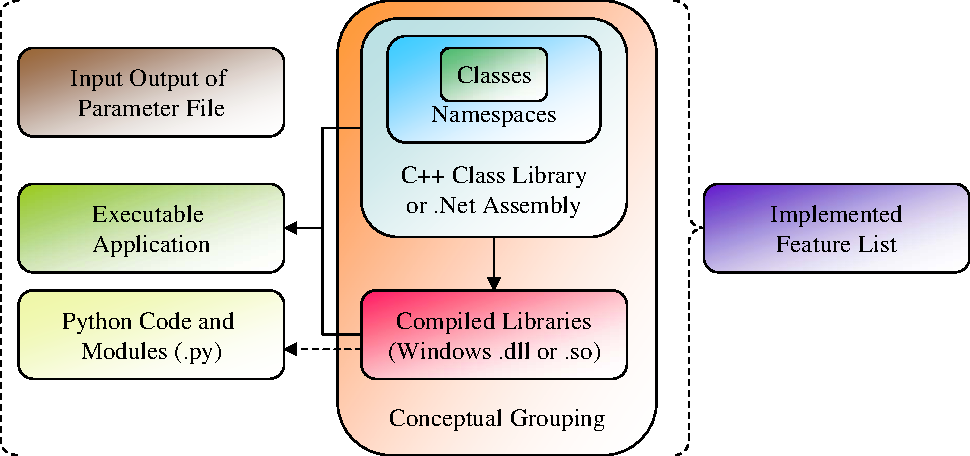
\includegraphics[width=0.8\textwidth]{03-Software/key/key.pdf}
\end{center}
\caption{The key for the conceptual software diagrams presented throughout the remainder of this chapter.}
\label{fig:software:conceptkey}
\end{figure}

We have already discussed the technical terms compilation, binary, executable and class. In addition to this a \emph{namespace} is simply a logical grouping of classes; two classes can share the same name as long as they reside within different \emph{namespaces}. Classes themselves can be distributed together in the form of a single library file as opposed to individual source code files. The subsequent compilation of such a compiled library results in a .dll (dynamic link library) file under Windows or a .so (shared object) file under Linux. Both of these essentially fulfil the same role of supplying a single logical code-base to multiple applications. Such compiled code can also be used by Python scripts, but requires non-trivial wrapper-code to import functionality. Class libraries for Microsoft's \dotnet\ also use the .dll filename extension and essentially perform the same role, but  work in a completely different way internally, meaning the two types are not compatible.


\clearpage
\section{PD}
\label{section:software:pd}

\pd\ is the name for the novel simulation framework developed, from the ground up, for this work in collaboration with Mike Tyka. 
\pd\ was developed with several principle objectives:

\begin{description} \isep

\item[Rapid and Easy Development] The central purpose of \pd\ is that it
should facilitate rapid algorithm and methodology development. 
\item[Coding Standards]
OOP principles should be used extensively throughout development.
Thus, all core concepts should be abstracted into a series of  highly-modular and intuitive base-classes. The number of base-classes should be minimised for simplicity, but remain representative of all common usage. Example class structures should be provided to guide novice programmers into the internal structure of \pd.
\item[User Interface]
Each component should be made completely
available to the user, through a powerful scripting interface, so that they can be logically recombined to form novel algorithms.

\item[Generality] \pd\ should provide a framework on which a very broad variety of applications in computational chemistry and biology can be built. It should presume as little as possible about the nature of the molecules to be simulated,
or indeed the nature of the simulation.
It is a core design decision that parameters are \emph{never} hard-coded. 

\item[Execution Efficiency] Many features in a simulation framework like  PD require high efficiency of simulation.
Importantly, these features \emph{must} all be implemented in a well established \emph{compiled} language.
As long as standard coding practices are used, this should allow both out-of-the-box efficiency and significant scope for optimisation.

\item[Platform Independence] It is important that \emph{only} ANSI/ISO standards are used for all code. 
Code must be both platform and compiler independent, which should make \pd\ intrinsically portable.

\end{description}



\subsection{Implementation}

Fundamentally, \pd\ is the conceptual unification of a high performance molecular mechanics library called \mmlib,  written predominantly in \CPP\ and exhibiting an automatically generated Python wrapper. Essentially, to use \pd\, the user simply writes a short
Python script which invokes functionality within \mmlib.

Python is intrinsically superior to the custom scripting engines used in other molecular mechanics frameworks like \amber\ and \charmm.
By contrast, applications written in
pure \CPP\ are capable of extremely high performance. The converse is not true. The performance of Python does not match that of \CPP. \CPP\ requires compilation and is therefore  intrinsically unsuitable as a scripting language. The solution to this conflict is a cross-language bridge, where code-division aids the fulfillment of the principle objectives. 

A potential disadvantage of defining \CPP:Python bridge-code
is increased developer overhead -- in fact this is a problem with the competing package \textsc{Ball}. In \pd\ this is completely avoided via automation of the wrapping process.
 The entire Python interface  is created automatically by an open source application called SWIG\cite{COMP:SWIG}.
Importantly, Python, SWIG and a host of efficient \CPP\ compilers are available for virtually all major operating systems and architectures.
Figure \ref{fig:software:pdusage} illustrates the interplay between the various framework elements. Primary usage is illustrated in the central grouping.

\begin{figure}[htbp]
\begin{center}
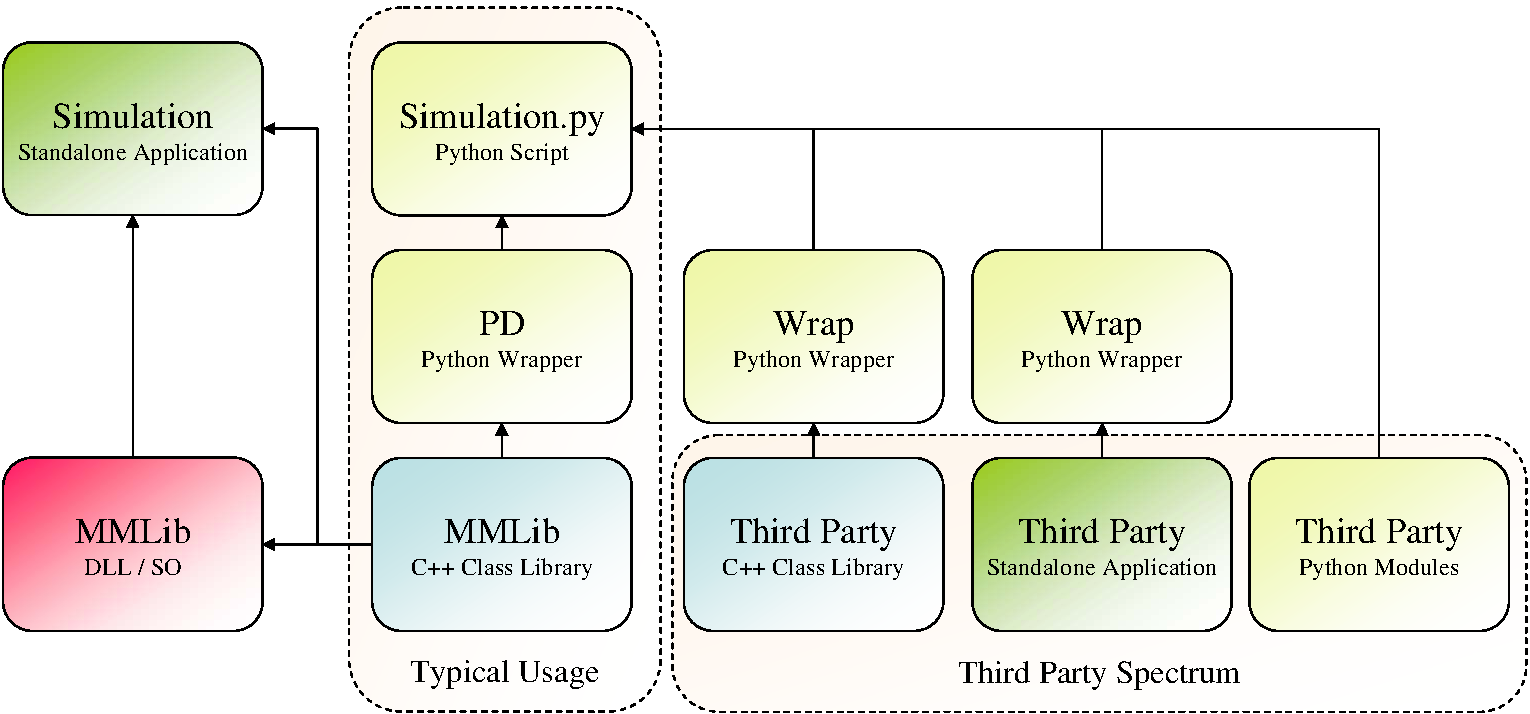
\includegraphics[width=0.95\textwidth]{./03-Software/pd/pd_framework.pdf}
\caption{Overall PD Structure and linking opportunities.}
\label{fig:software:pdusage}
\end{center}
\end{figure}




\subsubsection{The Core Library: MMLib}

The underlying framework of \pd\ is called \mmlib\ and coded in pure \mbox{\CPP.} \mmlib\ uses 
a \emph{minimal} series of abstract base classes to describe key ideas, which are are defined in section \ref{section:software:pd_code_overview}.
These base-classes are intuitive, well defined and interact in a modular manner. 
As most execution time is spent in the inner loops of forcefield calculations,
the use of this high-level abstraction comes with no measurable performance loss.
It is the view of the developers that this modular paradigm fits perfectly into the research environment.

Internally, \mmlib\ adopts standard OOP practice including industry standard design patterns,
pure ANSI \CPP\ and heavy use of the STL (the \CPP\ standard template library); which makes the code intrinsically
portable.
Although OOP principles are used throughout \pd, an important design choice was not to over-use
highly technical and non-intuitive code patterns. By keeping code inter-relationships
more simple there are a number of advantages. Primarily, over-complication
would go against the principle design ideals of \pd\ --  such practice
makes the code more difficult to understand and therefore makes algorithm
development \emph{less} rapid. Secondly, some language features (such as
virtual function calls), if used
inappropriately, can result in a significant performance penalty.




\subsubsection{The Python Interface}


Python is a fully-featured, well established, programming
language in its own right. A wealth of documentation and tutorials are available on the internet, meaning that the language is easy to learn for new programmers. All standard OOP constructs are available in addition
to the principle elements of procedural code such as arrays, conditional
statements and loops structures. These features are all far in excess of what you would expect to find built
into the input script parsers of the \amber\ and \charmm\ frameworks.
Python can also be used to completely replace traditional shell scripts in
terms of multiple job management. 

 
\pd\ takes integrated scripting to a new level. In addition to the rudimentary commands provided by other simulation engines, \pd\ provides all the basic building-blocks to formulate complex algorithms in abstract terms \emph{at the scripting level}. As the entire usable code-base is wrapped and exported automatically as a Python module, the latest features are \emph{implicitly} available to the Python user. Virtually every feature available by direct use of the underlying \CPP\ framework
is available through the Python interface.  By contrast to command-line flags, a Python interface vastly reduces the amount of manually written code necessary to expose available functionality. Not only is this incredibly powerful, but also extremely easy, freeing the programmer to worry less about code architecture and more about what he would like to accomplish. Use of the Python interface requires no recompilation --
it is often of benefit to be able to implement and tweak algorithms
in Python without the need to constantly recompile base-code.

In this
way
all the advantages of a custom scripting language are maintained as the
interface remains simple; however, as the user becomes more advanced, all
of the underlying functionality is available which allows complex algorithms can be created. For large developments, developers can add to the underlying \CPP\ framework
itself, whereby  their efforts will be \emph{implicitly} exported to the public Python interface for others to use.



 



 
 


\subsubsection{Alternative Code-base Access}

Typical usage of \pd\ is through the Python
interface, however, it is worth mentioning at this stage that although Python was chosen for
this work, SWIG is also capable of exporting for other common languages
such as TCL, Perl, PHP, and \CS\ (the \dotnet).

 
  
Figure \ref{fig:software:pdusage} also shows how the functionality of \mmlib\ can  be extended through
three potential Python-related paths. Python is sometimes described as having ``batteries included''. That is
to say, a great deal of third party functionality is available, very often free of charge, in what are called Python modules. These features can all be directly imported
into Python scripts. This includes modules for numeric analysis, SQL database interaction, networking, web services, graph
plotting and even OpenGL (3D Rendering). Secondly, entire third party applications could potentially be invoked via a Python-based manager. The subsequent output would be parsed and returned to the main script. Finally, just as with \mmlib, any other \CPP\
code library can also be wrapped using SWIG to make its functionality available.


The result of such modularity is that one could create, with minimal new code, an application which: loaded a series of  PDB identifiers from an\ SQL database; downloaded the files;  performed molecular dynamics simulations; all whilst plotting a graph of the energy. One such planned amalgamation
is an interface between \pd\ and \pymol; a very powerful and well-established molecular
graphics viewer, written mainly in Python, and free for academic use. This would give \pd\ very powerful graphical capabilities as well as greatly extending the simulation capabilities
of \pymol.

The Python interface is not the only way that functionality within \mmlib\ can be accessed --
two additional routes exist. The first is to statically link the \CPP\ class library
directly into a stand-alone simulation executable  which would perform a
specific function, but use the functionality within \mmlib. A second option
is the creation of a .dll file under
Windows or a .so file under Linux, which can be dynamically linked against other applications to give them bio-simulation capabilities.



\subsection{A Real-World Example}


The best way to illustrate just how well the small number of base classes
that \pd\ uses are able to very concisely describe typical molecular simulations is to show an example.
Each class has a clear purpose and each links into the next, ultimately  defining the  simulation.
Each of the code-boxes below represents a  section of the same python script.
Each section is discussed in turn. 

\lstset{language=Python} % For all listings in this enumerations
\begin{enumerate} \isep

\item The first thing one needs to do in any python script is to import all
required modules. As we are only defining  a simulation, all that is needed is the \pd\ module.

\begin{lstlisting} 
from pd import *                   # Load the pd module!
\end{lstlisting}

\item Next  \pd\ format forcefield parameters are loaded. These are contained within a parameter file that
describes both molecular topology and parameters for various
energetic forcefield components; previously described in section \ref{section:protmodel:energy_functions}. The topology is essentially
a list of named molecules, their atoms and associated properties.
\begin{lstlisting}
ffps = FFParamSet()
ffps.readlib("amber03aa.ff")       # Load the standard AMBER ff03 parameters
\end{lstlisting}

\item The forcefield parameters are now passed to a newly created \textsl{System} class which can represent any molecular system. Internally, it contains a
number of hierarchical dynamic arrays which contain \textsl{Molecules}  and functions required for their manipulation. In the example below we
use PDB\_In which \emph{derives} from System, augmenting it with the abilities to
read molecules from PDB files.

\begin{lstlisting}
sim = PDB_In( ffps, "myprotein.pdb" ) # PDB_In is a type of System
sim.load()                            # Load everything from the PDB file
\end{lstlisting}

\item The primary purpose of the \textsl{System} is to represent molecules in a hierarchical
manner, which makes manipulation of the underlying system more simple, for
example it is very easy to duplicate molecules. A hierarchical representation
however does not lend itself to efficient computation -- for this a more classical
linear array of atoms is required. This is provided by the class \textsl{WorkSpace},
which is generated from either the entire system or a defined sub-section which
requires efficient simulation. Such a sub-section could be a surface loop and
surrounding protein core residues.
Each of the appropriate atoms is then replicated within the \textsl{WorkSpace}.

\begin{lstlisting}
wspace = WorkSpace( sim )
wspace.info()                     # Prints a small block of info about the contents    
\end{lstlisting}

\item A \textsl{Forcefield} is now required to describe the energetics of the system.
In the example below we add the standard \amberff\ bonded forcefield and
a simple non-bonded forcefield with VDW\ interactions and vacuum electrostatics. \pd\ also implements many other more sophisticated forcefield components beyond the scope of this discussion.  

\begin{lstlisting}
ff = Forcefield(wspace)           # Initialise a Forcefield container with a link to 
                                  # a WorkSpace instance
bonded = BondedForcefield()       # Create the bonded forcefield component
nonbonded = NonBondedForcefield() # Create the non-bonded forcefield component

ff.add( bonded )                  # Add both to the parent container
ff.add{ nonbonded )               # 

ff.info()                         # Print the energetics of the pre-simulation system
\end{lstlisting}

\item In this particular example, the user wishes to perform a 1,000 step
conjugate gradient energy minimisation. We simply create an instance
of the \textsl{Minimisation} class.

\begin{lstlisting}
min = Minimisation( ff )          # Tell the minimisation what its forcefield is
min.Steps = 1000                  # Change the number of steps from the default to 1000
min.UpdateScr = 10                # We choose to update the screen every 10 steps
\end{lstlisting}

\item We may also decide that we wish to monitor changes in a given set of system properties, such as structural deviation from the starting conformation. As such,
one or more \textsl{Monitors} can be added to the simulation. \textsl{Monitors} can include
those for energy terms, RMSD values and other geometric quantities. After such
monitors have collected data, multiple statistical quantities can be requested.

\begin{lstlisting}
mon = CRMSMonitor( wspace )       # Create a new cRMS Monitor
min.addMonitor( mon )             # Add it to the simulations monitor container
\end{lstlisting}

\item Finally, we execute the simulation. The requested 1,000 steps of energy
minimisation are performed and  the screen is updated with energetic
information. 

\begin{lstlisting}
min.run()                         # Execute the simulation
\end{lstlisting}

\item Once complete, we can ask the Forcefield to print an energy
report and the monitors to show their measurements. 

\begin{lstlisting}
ff.info()                         # Print the energetics of the post-simulation system

mon.printHeader()                 # Print a nicely fomatted title
mon.printCurData()                # Print the curent cRMS
mon.printHistogram(0.1)           # Print a histogram of the recorded data
\end{lstlisting}

\end{enumerate}

So in only 23 code lines, we have represented and executed a complex energy minimisation,
reporting only the data that was relevant to the user. Even though this
script is short, it embodies almost every major aspect of \pd\ and illustrates
the use of 7 of the 10 primary base-classes.

The defining feature of the \pd\ Python interface is that it is clear, intuitive and
human readable; especially in comparison to
the equivalent \charmm\ script (listing \ref{listing:software:charmm}, discussed in section \ref{section:software:prob4progflow}) which doesn't have the same extensibility or
encapsulated data monitoring capabilities. Legacy custom scripting languages  also tend to
use rather cryptic commands such as ``hbuild sele all end'' which make incomplete sense without complementary well-written  documentation.
It is, therefore, the view of the \pd\ developers that \pd\ has features which are unprecedented in comparison to all older frameworks. This   makes \pd\ \  clearly superior in terms of user interaction.

\subsection{Fundamental Class Overview}
\label{section:software:pd_code_overview}

In the following section, a \emph{brief} overview of the defining elements
of \mmlib\ will be presented along with simplified typical usage. Figure
\ref{fig:software:pdclasses} shows the primary class relationships within
\pd\  (although there are others) which will be described below.

\begin{figure}[htpb]
\begin{center}
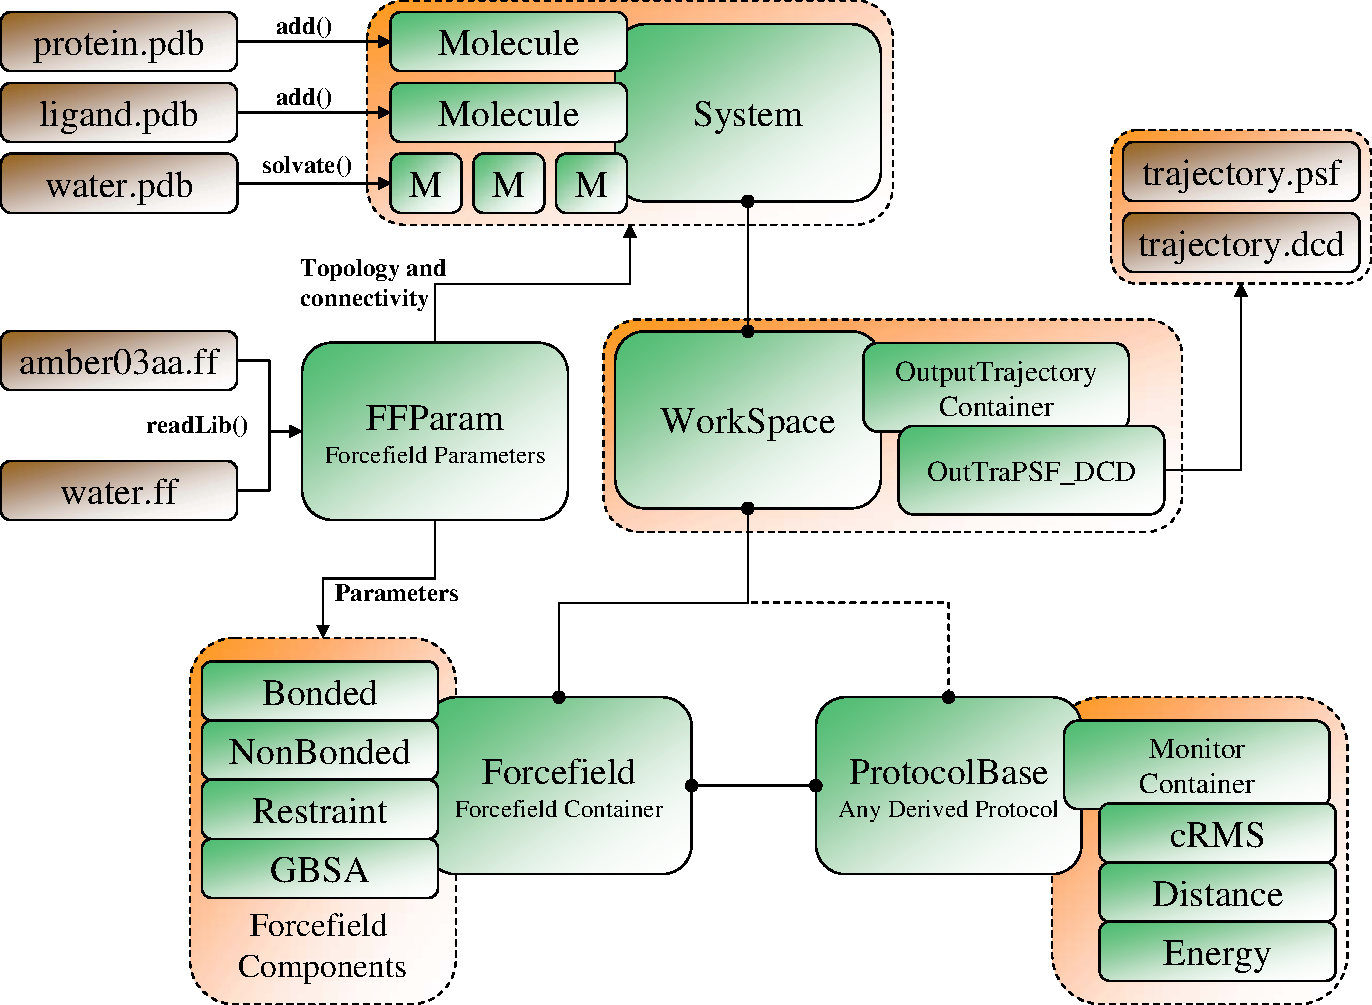
\includegraphics[width=0.95\textwidth]{03-Software/pd/class_Relationship.pdf}
\caption[\pd\ base-class relationships]{\pd\ base-class relationships. System is used to manipulate the pre-simulation molecular state. The central triad of the \textsl{WorkSpace}, Forcefield and \textsl{ProtocolBase} are used to embody the simulation itself. The various leaf elements and files are used to either import or export information.}
\label{fig:software:pdclasses}
\end{center}
\end{figure}

\subsubsection{A Consistent Model}

To reduce the learning-curve for both the use and development of \pd, it is important to maintain consistency
between different aspects of the framework. 
One such common theme throughout \pd\ is an abstract base class, with complementary
collection class. This statement might seem complex, but is actually quite
simple and is defined below.

In section \ref{section:software:inheritance} inheritance and its advantages were briefly discussed, along with a definition for the term base-class.
An \emph{abstract} base class is essentially the same, but does not implement one
or more of its member functions. You can never create an object from an abstract base class, you can only derive form it. Classes which derive from abstract base classes
must implement the missing functions, or they remain abstract themselves.

This concept makes sense in \pd: An excellent example for the use of an abstract base class in \pd\ is \textsl{ForcefieldBase}, which embodies the concept
of a forcefield component. Every derived forcefield component \emph{must} implement
the function calcEnergies(), which of course cannot be done until one knows
exactly what the component does. Each forcefield component does, however, share a good
deal of common functionality, including the need for addition into a common forcefield
container to perform its function. Another perspective of this is that, once a programmer has derived from \textsl{ForcefieldBase} and implemented all the required functions, his class is guaranteed to fit into the framework and can therefore
be used with all other available functionality.
 
Secondly, the \textsl{Forcefield} class \emph{is} simultaneously a
collection class and a type of \textsl{ForcefieldBase}. The role of the \textsl{Forcefield} collection is to hold other forcefield components. When the  \mbox{calcEnergies()}
function of the collection is called, it simply sums the return value of the \mbox{calcEnergies()} call
for each of its children. As such, the Forcefield container itself may be added
to a parent Forcefield container and thus forcefields can be \emph{managed as groups}, adding hierarchical flexibility to the framework.

The paradigm
of an abstract
base class and a container class which itself derives from that base is used again and again for each of \textsl{MoveBase},
\textsl{FilterBase}, \textsl{MonitorBase} and \textsl{OutputTrajectory}.

\subsubsection{FFParamSet}

\textsl{FFParamSet} is a \emph{run-time} database of chemical information and complementary
simulation parameters. Following creation of the class instance, data is imported form one or more \pd\ format ``.ff'' files, which are inspired by the
\charmm\ format, but borrow some superior elements from other formats. Code to parse the\  \charmm\ forcefield
format itself is, at the time of writing, undergoing further development. This additional parser implicitly extends the available forcefield sources
for \textsl{FFParam}, as many varied forcefields are already publicly available in
\charmm\ format, such as the \textsc{Opls} \forcefield. 

Once data is loaded, definitions are present for the chemical make-up of
polymers, residues and atoms. These data include atomic types, connectivity, radii, force constants, torsional parameters, amongst specific parameters
for individual specialised forcefield components. Robust data parsing is one of the most code-intensive activities within a given framework.  
As all simulation parameters can be loaded and stored via this class, which also facilitates subsequent structured
data access, no other components ever need to parse their parameters from separate files.
This greatly reduces the amount of IO code required and therefore reduces
both code complexity and maintenance requirements.

\subsubsection{System}

A \textsl{System} class is a container for the class \textsl{Molecule} and contains functions
concerned with the forcefield-independent geometric manipulation and duplication
of these
molecules. \textsl{Molecule}, in turn, owns both atom coordinates and properties.
Importantly, \textsl{System} is a hierarchical container representing intuitive relationships between chemical entities. All connectivity information is supplied by the \textsl{FFParamSet} class instance which is passed to \textsl{System} in its constructor. 


\subsubsection{\textbf{FileInBase}}

\textsl{FileInBase} is an abstract base class which derives from system, representing a file format which
contains molecular information, such as the PDB format. As an \textsl{FileInBase} \emph{is a} \textsl{System}, it merely adds functions that can import molecules from a file, but is essentially used as a standard \textsl{System} instance.

\subsubsection{WorkSpace}

The \textsl{WorkSpace} is always created from a \textsl{System} and is intended to hold the current simulation state. Potentially, multiple \textsl{WorkSpaces} can be created for a given \textsl{System}, in a one-to-many relationship. A practical example of this could be in protein surface remodelling where
each loop could be treated as a separate \textsl{WorkSpace} with minimal surrounding
atoms.

Each atom has properties
like Cartesian position, force and velocity, which may or may not be used
in use for a given simulation. Importantly, it is the classes that derive from \textsl{ForcefieldBase} and \textsl{ProtcolBase} which are allowed to modify these properties. The \textsl{WorkSpace} retains an internal link to its parent \textsl{System}, so that \textsl{System} properties can be updated following simulation. 

The \emph{critical} aspect of the \textsl{WorkSpace} is its internal linear atom array,
which is the primary distinction from the \textsl{System} class. This
concept allows in-code logic optimisations, but also critically benefits
the highly-optimised memory pipe-lines of modern computing architectures. Briefly,
memory is brought to the processor in \emph{pages}, which are defined as
short sections of contiguous memory. If memory is requested outside this range, then the processor must wait for it to be delivered, drastically reducing performance. By ensuring that the underlying memory is contiguous -- \ie\ the linear atom array -- the computers paging operations become more
efficient and thus execution times are reduced. 

\textsl{WorkSpace} supplies a number of additional plug-in components, each of which
provides easy access to pre-defined information regarding the nature of the
underlying molecular system. These include
the \textsl{BondOrder} array, which defines the order of the connectivity between
atoms in the \textsl{WorkSpace}; the \textsl{NeighbourList} which stores information as to
which atoms are proximal to one another; the rotatable bond array,
\textsl{RotBond},
which dictates which bonds can be rotated within a torsional representation;
and finally the \textsl{OutTra} container which can hold one or more output trajectory objects of any defined format.
\textsl{WorkSpace} also supplies a vast variety of functions to alter the Cartesian
and torsional states of the molecules that it contains.

\subsubsection{ForcefieldBase}

Each \textsl{ForcefieldBase}-derived class represents a forcefield component. When it makes sense
to do so, for example if it is more computationally efficient, some related
components are calculated together. An  example of this is the bonded forcefield components described in section \ref{section:protmodel:bondedterms} and shown as a single unit in figure \ref{fig:software:pdclasses}.

Each derived class 
is ultimately going to implement  two key functions; \mbox{calcEnergies()} and, if it is capable of supplying first derivatives, also \mbox{calcForces()}.
All parameters for execution are supplied by the \textsl{FFParamSet} instance passed
to the component when it is created. Following execution of these statements, the variables holding energetic terms within the \textsl{WorkSpace}
are incremented and the forces summed onto each atom's current force. It is
the Forcefield container class which is responsible for invoking the calcEnergies()
or calcForces() of each of its subordinate \textsl{ForcefieldBases} \emph{when directed} by the currently active \textsl{ProtocolBase}. 
 



A useful feature is that individual forcefield components can be activated
or deactivated as the user sees fit during execution. Additional \forcefield\ components
can also be added at any time as the user sees fit. This gives the user full
control over the progression of the simulation. Individual components can
also be made passive, whereby they do not contribute to the energy of the
system. This can be useful if one wants to monitor what the value of a given term would be, whilst not wanting to influence the active \textsl{ProtocolBase}. 

It was discussed in section \ref{section:protmodel:comparativemodellingarchetypes},
that the most successful comparative modelling methods are those which can include a variety of experimentally and statistically derived restraints. The modularity of the forcefield component paradigm used in \pd\ lends itself
perfectly to this, as forcefield components can be dynamically added for any imaginable
restraint or constraint. 

\subsubsection{ProtocolBase}

Classes derived from \textsl{ProtocolBase} are responsible for moving atoms in the
\textsl{WorkSpace} in response to the energies and forces described
by the \textsl{Forcefield}. As such, the \textsl{ProtocolBase} is essentially at the core
of the entire simulation. The simulation behaviour is provided by the implementation
of the function run\_core(), which makes all the decisions.
Each protocol owns a \textsl{MonitorBase} container which monitors the
result of its activities.

The basic set of implemented protocols is essentially most of the conformational search algorithms
defined in section \ref{section:protmodel:conformational_search}, along with other
techniques such as energy minimisation and higher-level protocols for loop
building and protein docking. These basic protocols do not have to act alone, but can be nested, partnered and extended by the user to
create novel kinds of simulation. Importantly, it is the common interface\ which allows this to work, as by definition all protocols must implement run\_core().
Good examples of how this can be done
are described later in section \ref{section:software:extendpd}.

 
\subsubsection{MonitorBase}

The idea of a Monitor is a very low-level abstract concept. As such, classes
which derive from \textsl{MonitorBase} really can monitor any quantity.
Each derived class simply implements the function setcurdata(), which is required
to set
a single member variable to the value of the measurement. The remainder of the functionality, such as producing histograms, calculating statistical properties and  printing
data is all provided by the base class. Creation of a new Monitor is trivial
as only one function need be implemented.

 
The measurements themselves are directed by the parent \mbox{\textsl{ProtocolBase}},
which informs its \textsl{MonitorContainer} to sample at a defined interval throughout
the simulation. As per the \pd-standard paradigm, the container is then responsible
for calling the measure() function of its children, causing them in turn
to call their own setcurdata(). This process results in a neat and intuitive
division of labour and a clear order of power.

\subsubsection{MoveBase}

Classes which derive from \textsl{MoveBase} are useful to a more limited set of \textsl{ProtocolBase}
classes which utilise discrete moves within their conformational search.
An example of such a class is  \textsl{MonteCarlo}. This Protocol owns a
\textsl{MoveBase} container (the paradigm returns) and calls each contained move in turn during the course of the simulation. Such moves could include Cartesian perturbations, torsional perturbations and rotamer assignments, as well as other more specific kinds. The exact composition is always defined by the users requirements.

\subsubsection{PickBase}

Some \textsl{ProtocolBases} use atom pickers, which derive all from \textsl{PickBase}.
These classes simply implement a single function which takes a reference
to a given atom and returns true or false as to wether that atom is within its
selection. Figure \ref{figure:software:pickingvenn} illustrates how basic pickers can be easily combined. As the protocol \textsl{PickedMinimisation} has been
implemented, this selection of pickers could be used, for example, to resolve \sidechain\ steric clashes in the N-terminal section of a protein model, without disturbing the remainder of the model. 

\begin{figure}[htpb]
\begin{center}
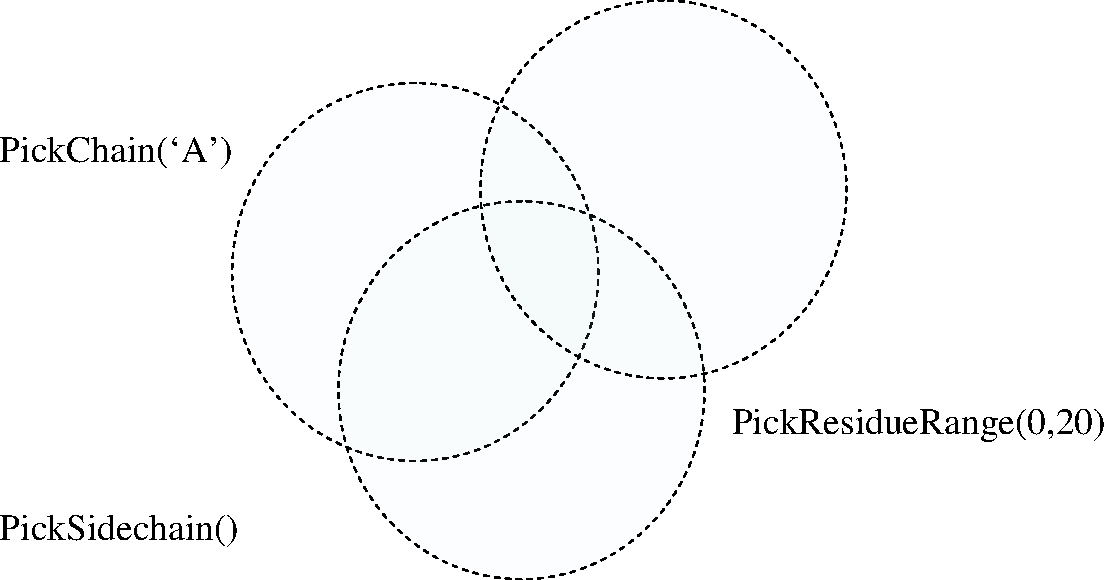
\includegraphics[width=0.7\textwidth]{03-Software/pd/picking.pdf}
\end{center}
\caption[Atom Picking in \pd]{A venn diagram showing how 3 basic pickers can
be combined to select only the \sidechain\ atoms of the 20 N-terminal residues of chain A.}
\label{figure:software:pickingvenn}
\end{figure}


\subsubsection{FilterBase}

\textsl{FilterBase} is intended as a mechanism to improve the sampling efficiency
of a given \textsl{ProtocolBase}. In some cases, especially when
large conformational change \textsl{MoveBases} are utilised, non-sensical conformations
can be generated during a simulation. As the main forcefield calculations are comparatively expensive,
it can be helpful to pre-screen conformations, only performing the  full evaluation on those which pass all filters.
Good examples of such filters are hard-sphere steric filters in MC simulations,
a bond-length filter, or a filter that tests to see if the \Omg\ peptide-group
torsion is within a given tolerance of 0\degree\ or 180\degree.  

\subsubsection{OutputTrajectory}

Output trajectories capture snapshots of a given workspace as directed by
the active \textsl{ProtocolBase}. As usual, these classes derive from a single class called \textsl{OutTraBase}, 
which embodies the basic properties of a trajectory such as the file-stem. It has already been stated that the 
\textsl{WorkSpace} owns an \textsl{OutTraContainer} object, which is commonly called by instances of \textsl{ProtocolBase}.  


\subsection{Examples of Extending PD Functionality}
\label{section:software:extendpd}

The aim of the following section is to describe how \pd\ can be extended
both by the user and the developer and how the supplied class framework acts to supply maximum flexibility in this endeavour. By allowing extension
and reuse of existing elements, development time can be reduced. 



\subsubsection{Extension Using Python Code}

\pd\ can be extended at the user interface itself, via the nesting of existing protocols. Unlike other frameworks, this does not require a single line
of new \CPP\ code to be written. 

Take for example the \textsl{MonteCarlo} protocol, which has a vast number
of uses\cite{SIMULATION:MC}. In its simplest form, the \textsl{MonteCarlo}
algorithm makes conformational changes which are then evaluated by ``the evaluator''. The conformational changes are supplied by the \textsl{MoveSet,} which contains multiple
component perturbations added by the user. By default
the protocol functions by the standard Metropolis criterion of acceptance\cite{SIMULATION:Metropolis};
rejected structures are restored to their previous valid state. In the simple case,
the evaluator is a \textsl{ProtocolBase} which does nothing except trigger a \textsl{Forcefield} energy calculation.


The following examples assume that we have already configured a \textsl{FFParamSet},
\textsl{System}, \textsl{WorkSpace} and \textsl{Forcefield}; ignoring both
\textsl{Monitors} and \textsl{Filters,} although of course these could easily be added. In this example, we exploit the MC algorithm
to pack \sidechains.



\lstset{language=python}
\begin{lstlisting}[float=h] 
# Add together an appropriate selection of MoveBases
moveset = MoveSet(wspace)                     # An empty container...
moveset.add( SidechainRotamerLibMove( ... ) ) # add a low probability move
moveset.add( SidechainTorsionalMove( ... ) )  # than a high probability move

# Configure the simplest evaluator, a ProtocolBase 
# which triggers a forcefield calculation
evaluator = Energy(ff) 

# Create a MonteCarlo protocol instance
mc = MonteCarlo( evaluator, moveset )   # Giving it some moves and a Protocol by which to evaluate
mc.Steps = 200                          # Perform 200 MonteCarlo iterations
mc.TargetTemp = Temp(300)               # Simulate at a constant temperature of 300K

mc.run()                                # Lets go!
\end{lstlisting}

Now that we have created an underlying system, the user can begin to experiment
with many different options. Firstly, we can change the temperature profile
from static to a linear decay. 

\lstset{language=python}
\begin{lstlisting}
# Create a MonteCarlo protocol instance
mc = MonteCarlo( evaluator, moveset )   # Giving it some moves and a Protocol by which to evaluate
mc.Steps = 200                          # Perform 200 MonteCarlo iterations
mc.TargetTemp = TempLinear(300,10)      # Simulate at a constant temperature of 300K

mc.run()                                # Lets go!
\end{lstlisting}

The linear temperature regulator automatically scales the temperature factor
from 300K to 10K over the course of the 200 steps. Other temperature profiles
are implemented such as exponential decay. Thus, with a single code line change, we have now implemented Metropolis MC with simulated annealing. 

A second potential change is of the evaluator, which is invoked prior to the
decision as to wether a structure should be accepted. If large conformational
moves are used, an obvious choice is an energy minimisation. 

\lstset{language=python}
\begin{lstlisting}
evaluator = Minimisation(ff)            # Configure a minimisation

# Create a MonteCarlo protocol instance
mc = MonteCarlo( evaluator, moveset )   # The passed evaluator is now different...
mc.Steps = 200                          
mc.TargetTemp = Temp(300)  

mc.run()                                # Lets go!
\end{lstlisting}

Again, with a single code change, we now have a Protocol with completely different
properties -- we have implemented Metropolis Monte Carlo with minimisation\cite{SIMULATION:MCM}.
A similar nested protocol change would be to use Molecular Dynamics with
a small number of steps at the
evaluator, creating Hybrid Monte Carlo\cite{SIMULATION:HybridMC} -- again this
only requires minor changes to the code, but creates a completely different algorithm. 


Finally, we have mentioned that Python can be used as a replacement for shell
scripts for managing multiple complementary simulations. Both replica exchange
molecular dynamics and replica-exchange Monte Carlo, REMD\cite{SIMULATION:REMD} and REMC\cite{SIMULATION:REMC} respectively,
require the coordination and exchange of parallel simulations. For these, the management
and exchange logic would need to be implemented in Python; essentially the
algorithm controlling the
temperature and coordinate exchange. 
This should be done in a generic manner; REMD and REMC actually share a majority of the same Python code and like the MC examples the only real difference
is the choice of evaluator. This single simulation script, as opposed to using
shell scripts, puts all code in one place, making it easier to maintain and more powerful due to the specific
advantages of Python.




\subsubsection{Extending Using New C++ Code}

Although the recombination of features via the Python interface is incredibly useful,
completely new features and algorithms will always require new \CPP\ code. It is hoped that the comprehensive nature of the \pd s base classes will mean that no additional bases are required. Inheritance, described in section \ref{section:software:inheritance},
is therefore an important mechanism. 
 
 
 
 As discussed in section \ref{section:protmodel:stun}, STUN\cite{SIMULATION:STUN}
 is a method which shares a significant amount of functionality with the
 standard MC algorithm, differing only by its acceptance function. Because
of this, there is little point in creating new code for anything apart from the acceptance function itself. By \emph{deriving} from \textsl{MonteCarlo}, \textsl{STUN} gains all of its functionality and is allowed to replace or \emph{overload} the accept() function call with new logic, reusing all other
code.

An advanced topic that is used throughout \pd\ is \emph{multiple} inheritance.
Rather than deriving from a single base class, in some circumstances, it can be appropriate to derive from two or more. 
An example of where this could be useful involves a class which derived both from \textsl{MonitorBase} and \textsl{NormalMode} and adds a small amount of stitching-code. 
This hybridisation, via multiple inheritance, effectively defines a crude entropy monitor for use during the course of a given simulation.  


\subsection{The List of Implemented Features}

At the time
of writing, a large number of features have already been implemented in \pd\  and a significant amount of functionality is planned for imminent
implementation.
The features that are used in this thesis are only a subset of the available scope of \pd. 

\begin {itemize} \isep
\item{Forcefield Components}

    \begin {itemize} \isep
     \item\textit{Bonded:}    Harmonic bonds, angles, fourier harmonic torsions and impropers. 
     \item\textit{Non-Bonded:} Lennard-Jones, \vdw, simple electrostatics. Energy and force switching functions.
     \item\textit{Spaces:} Infinite vacuum, periodic boundary conditions (orthogonal)    
     \item\textit{Solvation:} Distance-dependent dielectric constant\cite{FORCEFIELD:DistDepDi}, solvent accessible surface area (SASA) based solvation including both Eisenberg et al.\cite{FORCEFIELD:SASA:Eisenberg} and Ooi et al.\citep{FORCEFIELD:SASA:Ooi}, POPS\ algorithm for SASA by pairwise distance approximation\cite{FORCEFIELD:POPS}, generalised Born / surface area (GB/SA) \citep{COMPCHEM:Still90,FORCEFIELD:Qui1997,FORCEFIELD:Zhang2003}.      
     \item\textit{Knowledge Based:} Residue:residue interaction-matrix.     
     \item\textit{Restraints:} Harmonic, Cartesian distance and torsional restraints. Miscellaneous custom forces.
     \item\textit{Other:} G\={o} type forcefield, soft-sphere VDW Forcefield
    \end {itemize}

\item{Forcefield implementations:}
        \begin {itemize} \isep
           \item\textit{\amber}:  ff94 \cite{FORCEFIELD:AMBER:94}, ff99\cite{FORCEFIELD:AMBER:99}, ff03\cite{FORCEFIELD:AMBER:03}   
           \item\textit{\charmm}\cite{FORCEFIELD:CHARMM}: \charmm-19, \charmm-22
           \item\textit{\opls}:   \opls/aa\cite{COMPCHEM:OPLS:C}
           \item\textit{Other}:   \textsc{Bude}\cite{THESIS:SOPHIE}, \raft\cite{COMPCHEM:Gib2001}
        \end {itemize}  
        
\item{Protocols \& Algorithms:}         
        \begin {itemize} \isep
           \item\textit{Gradient based Minimisation}: Steepest Descent, Conjugate Gradients and Torsional\cite{THESIS:BREWER}.               
           \item\textit{Monte Carlo}\cite{SIMULATION:Metropolis}: Monte Carlo with minimisation (MCM) \cite{SIMULATION:MCM} 
           \item\textit{Structural Perturbations}: A large variety including rotamer libraries\cite{COMPCHEM:RICHARDSON} and
          fragment insertions.  
          \item\textit{Comparative modelling}: Sequence alignment, threading, missing atom rebuild, \sidechain\ packing and loop modelling.          \item\textit{Conformational space annealing}\cite{SIMULATION:CSA}
          \item\textit{Molecular Dynamics}: Beeman \cite{SIMULATION:MD:Beeman}, Verlet and velocity Verlet integrators, Andersen \cite{SIMULATION:MD:Andersen} and Berendsen thermostats \cite{SIMULATION:MD:Berendsen}. (NVE, NVT and NPT).           \item Langevin Dynamics \cite{SIMULATION:Langevin}
           \item \textit{Replica Exchange Dynamics}  (REMD) \cite{SIMULATION:REMD}
           \item Numerical second derivate matrix (Hessian) calculation and normal mode analysis
           \item Quasi harmonic analysis \cite{SIMULATION:QuasiHarmonic,SIMULATION:QuasiHarmonic:B}
           \item\textit{Free-energy calculations}:  Free energy perturbation (FEP) \cite{SIMULATION:Zwanzig54}, thermodynamic integration \cite{SIMULATION:Kirkwood35,SIMULATION:Beveridge89}, umbrella sampling \cite{SIMULATION:UmbrellaSampling} and confinement methods \cite{THESIS:TYKA:PAPER06,THESIS:TYKA}
           \item Peptide \& protein docking\cite{THESIS:SOPHIE,THESIS:CRISP}
        \end {itemize}  
                        
\item{Monitors:}
        \begin{itemize} \isep               
          \item\textit{Structural deviation}: Cartesian and torsional RMSD measures
          \item Inter-atomic distances
          \item Native contacts
          \item Radius of gyration
          \item Energy components
        \end{itemize} 
        
\item{Rotamer Libraries:}
        \begin{itemize} \isep               
          \item Shetty\cite{NATIVE:Shetty2003}
          \item Rickardson\cite{COMPCHEM:RICHARDSON}
          \item Dunbrack\cite{NATIVE:Dunbrack2002} (Backbone dependent and independent)
        \end{itemize}
        
\item{Rotamer Packing:} 
        \begin{itemize} \isep               
          \item \textsc{Scwrl}\cite{METHOD:SCWRL_1,METHOD:SCWRL_2}
        \end{itemize}
                  
\item{Major file and trajectory formats:}
        \begin{itemize} \isep               
         \item PDB
         \item TRA (Bristol Trajectory Format)
         \item DCD \& PSF (used by \charmm\ and \namd)
         \item TRR \& XTC (Compressed trajectory format used by \gromacs)
        \end {itemize} 

\end {itemize} 





\subsection{Accessory Features and Advantages}

\pd\ as a framework comes with other implemented management features and benefits over
some other frameworks, including:

\begin{description} \isep
\item[Automatic Documentation] It is often said that the most up-to-date documentation is always the code itself. \pd\ uses the Doxygen code documentation system, whereby comments embedded within the code are parsed and corresponding documentation automatically generated. Output can be produced in many popular formats such as HTML and PDF. An excellent feature is that code-relationship diagrams are generated automatically and have hyperlinks allowing direct exploration of  code and associated comments. Currently such documentation is generated automatically on a nightly basis on the \pd\ web-server.
\item[Version Control] \pd\ is archived using Subversion -- an open source and well-supported version control system. As such, there is only ever one official version of \pd, whereby all developers work on their snapshot of the primary version and regularly commit updates. This greatly simplifies collaboration and implicitly documents all code changes and who made them.
\end{description}


\subsection{Benchmarks}

\pd\ is still in rigorous development and so far 
little time has been spent directly on code optimisation. Some
preliminary benchmarks have been made to test the feasibility of the underlying code-model.
Three separate benchmarks have been made against other respected packages, including \charmm\cite{FORCEFIELD:CHARMM}, Tinker\cite{COMPCHEM:TINKER}, NAMD\cite{COMPCHEM:NAMD} and Amber v8 (Sander)\cite{FORCEFIELD:AMBER}, and are shown in figure \ref{fig:software:pdbench}.

\begin{figure}[htbp]
\begin{center}
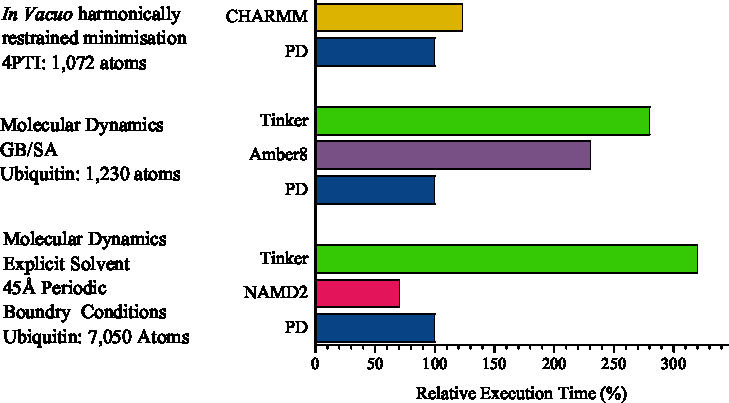
\includegraphics[width=0.9\textwidth]{03-Software/pd/benchmark.pdf}
\caption[Initial \pd\ Benchmarks]{Initial \pd\ Benchmarks. The MD data is reproduced courtesy of M. Tyka.}
\label{fig:software:pdbench}
\end{center}
\end{figure}

For a basic restrained minimisation protocol, \pd\ is shown to outperform \charmm\ version 3.0 (beta 2), reducing execution time by around 20\%. 
\pd\ also outperforms the Sander version of \amber\footnote{It should be noted that the Sander module
of \amber-8 is reported to be slightly slower than that of the newest GB/SA implementation in
\amber-9 (pmemd), which was unavailable within our group at the time the
benchmarks were computed. Thus, the performance of  \pd\ is most likely comparable to the latest \amber\ code.} and is competitive in execution time with \namd; each of which are respected applications in the
simulation community. \pd\ performs significantly better than \textsc{Tinker} on both MD examples, reflecting \textsc{Tinker}s lack of emphasis on raw performance.
The increased performance of \pd\ over \amber\ is attributed to code sections within \mmlib\ which have received most optimisation, especially
the GB/SA component. \namd\ is one of the most respected packages in terms of performance, having been developed by a large team for some time. It is therefore unsurprising that it outperforms \pd\ at the current time, although the relatively small difference is encouraging. It should
be noted that the periodic boundary code in \pd\ is still in developmental
form and lacks some of the most recent algorithmic enhancements that will
be present in \namd.


 \subsection{Concluding Remarks}


The main purpose of \pd\  is
as a highly flexible simulation framework. It is hoped that this overview has demonstrated that \pd\ achieves greater flexibility for the user than most competitors and where equal, already achieves 
higher performance. In addition, there is still significant scope for further optimisation.
Now that an impressive feature list has been implemented, the main development drive in \pd\ is now going to revolve around improvements for parallel architectures. Parallelisation has been planned since \pd\ was created, therefore whilst far from trivial to implement, there are no design choices which intrinsically prohibit parallel implementations.

The current \pd\ development snapshot at the time of writing comprises some 66,530 lines of in-house \CPP\ code, 7,809
lines of integrated third party code and 124,434 lines of automatically generated wrapper code.
It is clear that if the wrapping process were not automatic, it would represent a significant development burden.







\clearpage
\section{The UoB-Framework}
\label{section:software:uob}

As discussed, \pd\ is designed primarily as a simulation framework and so visual analysis tools are beyond its scope. In order to complement the simulation capabilities of \pd, it is also important to implement facilities for the extraction and subsequent processing of data from the PDB and other experimental sources. To this end, a second framework has also been developed in parallel, called the \uobf. It lacks simulation capabilities, but is instead concerned with error-tolerant data extraction and supplies many convenient methods for subsequent processing and visualisation. 

\subsection{Language Choice}

The \uobf\  has been developed \denovo\  using the \CS\ programming language\ and Microsoft's \textsc{.Net} framework on which it depends. As the \uobf\ does not provide simulation capabilities, the raw performance of the code generated from the language is less important. The language choice therefore stemmed from the superiority of \CS\ over the likes of \CPP\ for file processing and database interaction and over Python in terms of superior development tools. 


\subsection{Data Exchange -- Bristol Trajectory Format}

A new, storage-efficient, 
binary file format was developed in collaboration with Mike Tyka and Allan Brewer. All manner of energetic information 
is stored from the simulation that originally generated the file. 
This information is in excess of what is found in other file formats and varies dependent upon the exact simulation and 
\forcefield\ components loaded. The exact format is beyond the scope 
of this discussion, but is defined on the group web server. By standardising the format in which simulation data is stored, 
this data can easily be shared between applications that are produced within the research group.
Both \pd\ and \uobf\ are capable of reading and writing such files, as shown in figure \ref{fig:software:tra} 
-- the \uobf\ can then be used for simple visualisation, analysis and extraction of specific data produced by \pd\ 
simulations.

\begin{figure}[hptb]
\begin{center}
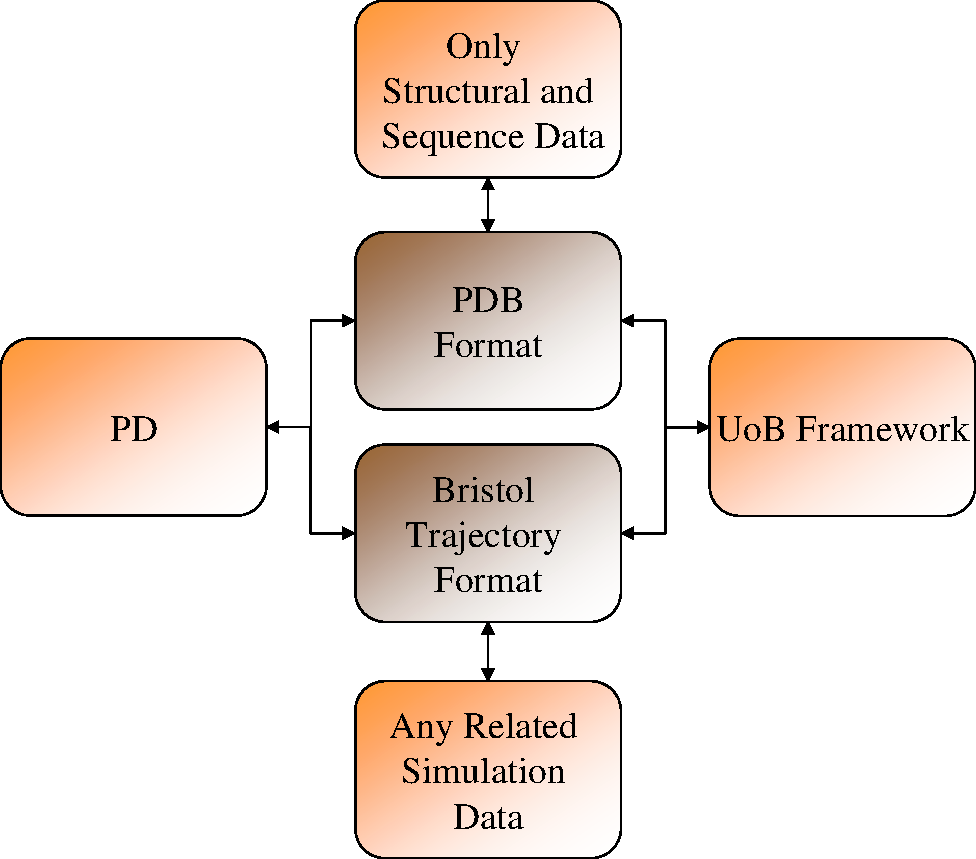
\includegraphics[width=0.5\textwidth]{03-Software/tra/tra.pdf}
\caption{Exchange and storage of data.}
\label{fig:software:tra}
\end{center}
\end{figure}


\subsection{Framework Structure}

The \uobf\  is highly modular in nature, comprising multiple  code assemblies which interact.\ These focus on the primary principles of flexibility and extensibility. The components can be rapidly intergraded into host applications for any given purpose, thus, the current implementation is used throughout this work. 

Figure \ref{fig:software:uobassemblies} illustrates that the \uobf\ is comprised of four primary \textsc{.Net} assemblies, each of which has a well defined role and is described in the following sections.

\begin{figure}[hptb]
\begin{center}
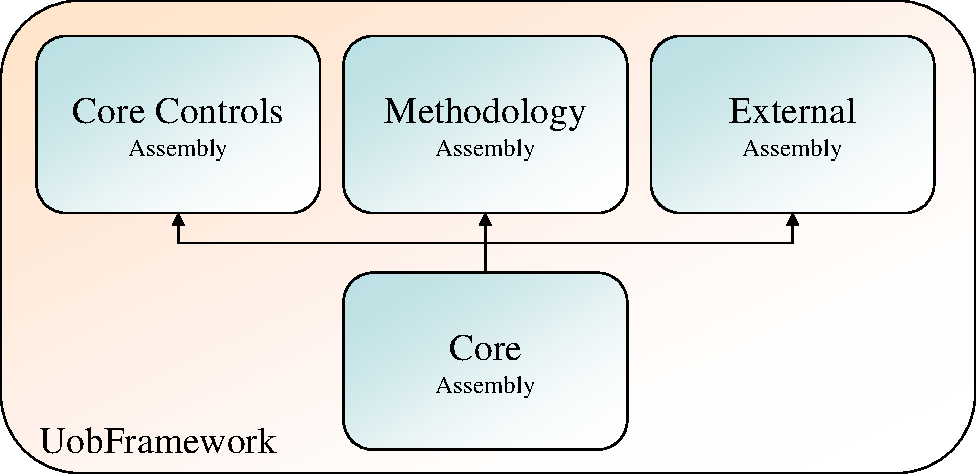
\includegraphics[width=0.5\textwidth]{03-Software/uobframework/assemblies.pdf}
\caption{The assemblies which compose the \uobf.}
\label{fig:software:uobassemblies}
\end{center}
\end{figure}

\subsubsection{The Core Assembly}
\label{section:software:uob:core_assembly}

Figure \ref{fig:software:uob:Core} shows a conceptual map of the functionality present within the core assembly of the framework. Structure and sequence data can be imported using functionality in the FileIO namespace. Development has focused on protein structures, however it could be easily extended to define other molecule types such as nucleic acids. Implemented structural manipulations include the rebuilding of missing atoms from library definitions and structural truncation and concatenation. Both structural and sequence alignments are available along with common functionalities like calculating sequence identities and \crms\ values. The data namespace is dedicated to the processing, statistical analysis and export of data. Finally, a number of additional tools are provided to simplify common labour intensive tasks. 

\begin{figure}[hptb]
\begin{center}
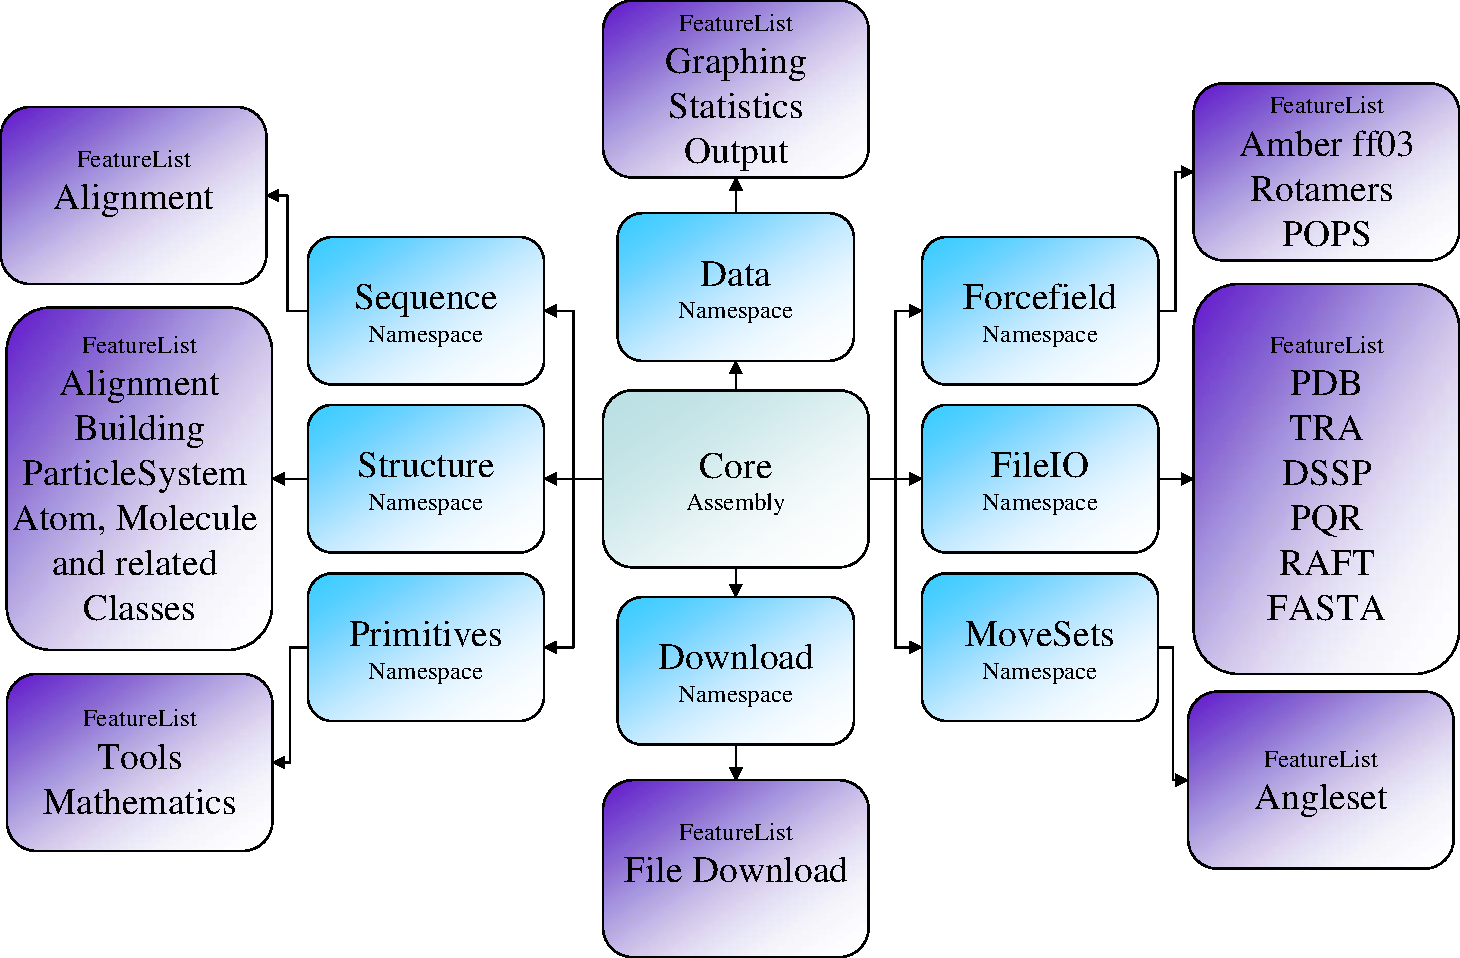
\includegraphics[width=0.75\textwidth]{03-Software/uobframework/core.pdf}
\caption{The component namespaces of the Core assembly and associated functionality.}
\label{fig:software:uob:Core}
\end{center}
\end{figure}

\subsubsection{The Core Controls Assembly}
Figure \ref{fig:software:uob:CoreControls} shows a conceptual map of the functionality present within the Core Controls assembly, which contains the visual components for user interaction with the Core assembly. This can be utilised by any application to allow user interaction with the underlying molecular data. Data visualisation is highly useful when analysing the large data sets that are typically produced during simulation.
The main included components are the molecular render controller and tool windows to control it; an associated OpenGL 3D graphics engine; and tool windows to control and display the underlying trajectory and  its data.
Each of these link together in a logical network, triggering each other to update as data is changed. For example, when the current trajectory position is changed using a trajectory control, it will  result in any linked OpenGL\ window refreshing to display the corresponding coordinates. 

\begin{figure}[hptb]
\begin{center}
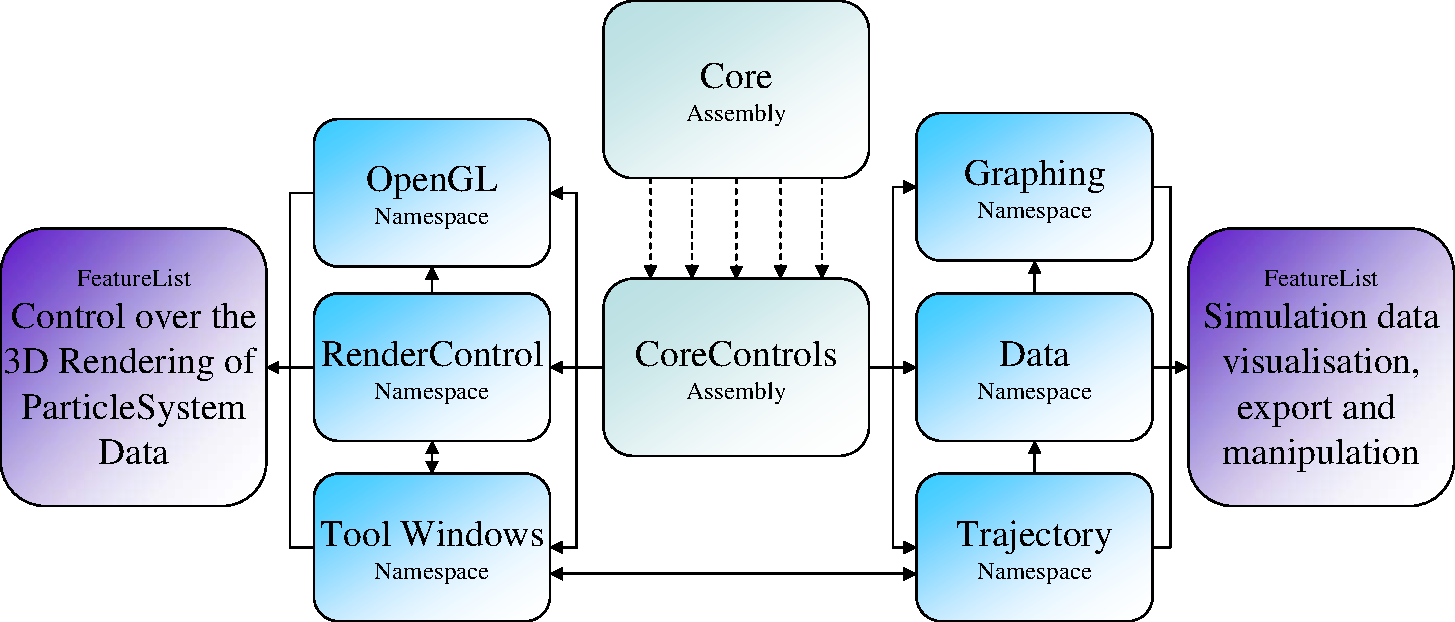
\includegraphics[width=0.75\textwidth]{03-Software/uobframework/corecontrols.pdf}
\caption{The component namespaces of the Core Controls assembly and associated functionality.}
\label{fig:software:uob:CoreControls}
\end{center}
\end{figure}

\subsubsection{The External Assembly}
The external assembly allows the \uobf\ to interactively distribute tasks to external applications. These applications are invoked asynchronously and their progress and data output is monitored. An example is the ability to launch an energy minimisation in \pd. By combining this with the core controls assembly, the   progress of the minimisation can be displayed and  minimised structure automatically imported for analysis. The external assembly also contains wrapper-code for a free file compression utility, therefore providing  an in-code user-friendly interface to any data stored within compressed files.

\subsubsection{The Methodology Assembly}
\label{section:uobf:methodology}

The Methodology assembly, shown in figure \ref{fig:software:uob:Methodology}, concerns the encapsulation a given task
into a class which derives from \textsl{TaskDirectoryInteration} and a set of complementary child classes. Each of these individual tasks is based around a single file-system folder  -- termed the Task Directory -- which may contain one or more libraries, a script generation folder, a result folder and a report folder. This system has been used throughout many of the developments in this work, including those in chapters \ref{chapter:database}, \ref{chapter:reduced_rep}, \ref{chapter:casp} and especially in \ref{chapter:methods}. Each application or application sub-mode uses a single Task Directory and performs its current operation upon it -- whether that be generating scripts to submit a simulation to a computer cluster, verifying produced data, fitting functions to data or producing reports based upon simulation output.

As discussed later in section \ref{section:loopcriterion}, \dssp\ has been used as the secondary structure annotation application throughout this work. As such, a common base class named \textsl{DSSPTaskDirectory} was derived from \textsl{TaskDirectoryInteration}, which is concerned with tasks that use a \dssp\ file library. Each of these tasks analyses some property that is contained within \dssp\ files, usually the \dssp\ secondary structure annotation, but sometimes useful auxiliary information such as \phipsi\ angles, SASA and per-residue temperature factor.


The final namespace is used to interact with a third party application called Origin, used to produce publication-quality statistical graphs. The classes within this namespace interact with the Origin's COM interface
in order to automatically produce reports containing graphs.
An example of such use is figure \ref{fig:intro:ramachandran}, which was actually originally part of an automated per-residue-type Ramachandran distribution analysis. The software engine for this analysis is contained within a class which derives from \textsl{DSSPTaskDirectory}. This then uses the Origin namespace to automatically produce both contour and scatter Ramachandran plots from the current database.

\begin{figure}[hptb]
\begin{center}
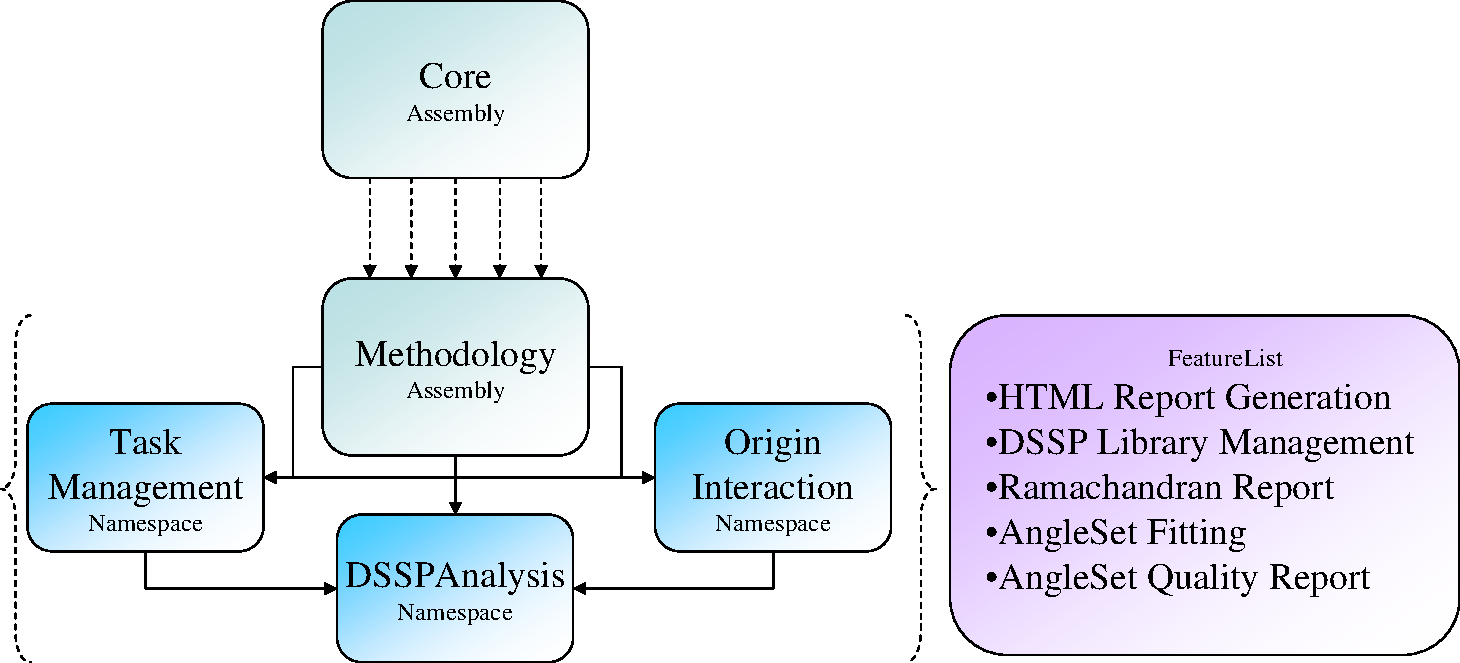
\includegraphics[width=0.85\textwidth]{03-Software/uobframework/methodology.pdf}
\caption{The component namespaces of the Methodology assembly and associated functionality.}
\label{fig:software:uob:Methodology}
\end{center}
\end{figure}

\subsection{Developed Applications}

Many applications have been developed which use the functionality contained within the \uobf\ and are listed in figure \ref{fig:software:uobapps}. These are discussed in detail in the relevant chapters of this dissertation. \dave\ is discussed briefly in the following section. A structural database creation engine named \pdbdb , is discussed in chapter \ref{chapter:database}.
The applications for \angleset\ viewing and fitting are discussed in chapter \ref{chapter:reduced_rep}. Finally, the ``Method Calibration'' software plays a critical role in chapter \ref{chapter:methods} -- without such software, the analysis would have been reduced to a convoluted set of hard-to-document shell scripts with poor error-checking.



\begin{figure}[hptb]
\begin{center}
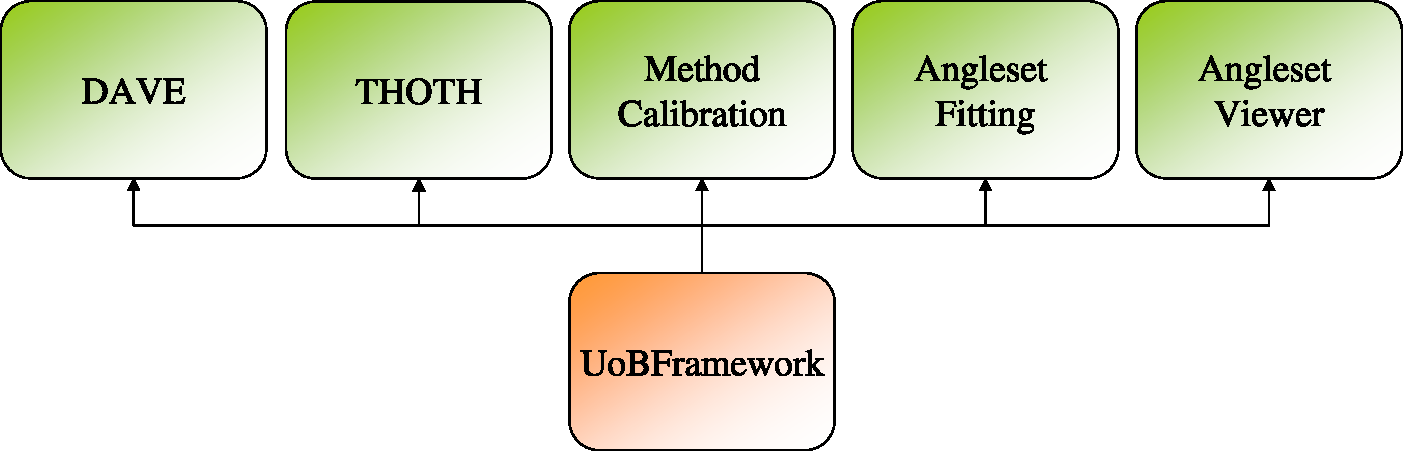
\includegraphics[width=0.8\textwidth]{03-Software/uobframework/apps.pdf}
\caption{The developed applications which rely on the \uobf.}
\label{fig:software:uobapps}
\end{center}
\end{figure}



\subsubsection{DAVE}

\dave, or Dynamic Atomic Visualisation Environment, is intended as a viewer of simulation data in its structural context. Importantly, \dave\ is not intended for use in the production of publication-quality molecular graphics, as there are many superior applications for this purpose. Instead \dave\ primarily deals with PDB and Bristol trajectory format files.

\dave\ possesses chemical knowledge of the molecules it is displaying, derived from a \pd\ format forcefield parameter file containing the \amberff\ definitions. As such, unlike in other viewers which must guess atomic connectivity and hence show incorrect bonding when close atomic contacts are present (common in unrefined models), \dave\ always displays the correct atomic connectivity. \dave\ can also display a tree-view for easy visualisation of any present polypeptides and provides drawing controls to change their appearance in the 3D display, both of which are side-bars in figure \ref{fig:software:davemain}. 

Any stored simulation data can be displayed directly in a simple data box, plotted graphically (figure \ref{fig:software:davegraph}) or exported in .csv format to applications like Microsoft Excel or Origin for further analysis. If the file was generated by \pd, there is also the option of displaying additional coloured vectors on the screen to represent arbitrary  aspects of the simulation. These lines are defined by the simulation and stored within the Bristol Trajectory format file. An implemented use of these lines is in displaying the force vector on each atom. They could also be used to display artificial inter-atomic restraints used during the simulation which are not part of the standard forcefield.

In addition to displaying pre-calculated information, \dave\ is also capable of its own analysis. One such display, which is generated on-the-fly, is the dynamic Ramachandran plot shown in figure \ref{fig:software:davemain}. As the current displayed simulation frame changes, the \phipsi\ angles are updated in the plot. 

Finally, \dave\ provides some more advanced tools including the ProSup structural alignment protocol\cite{COMPCHEM:ProSup}, launching an energy minimisation in \pd, displaying aligned sequence information and finally, a facility to rebuild missing atoms.

\begin{figure}[p]
\begin{center}
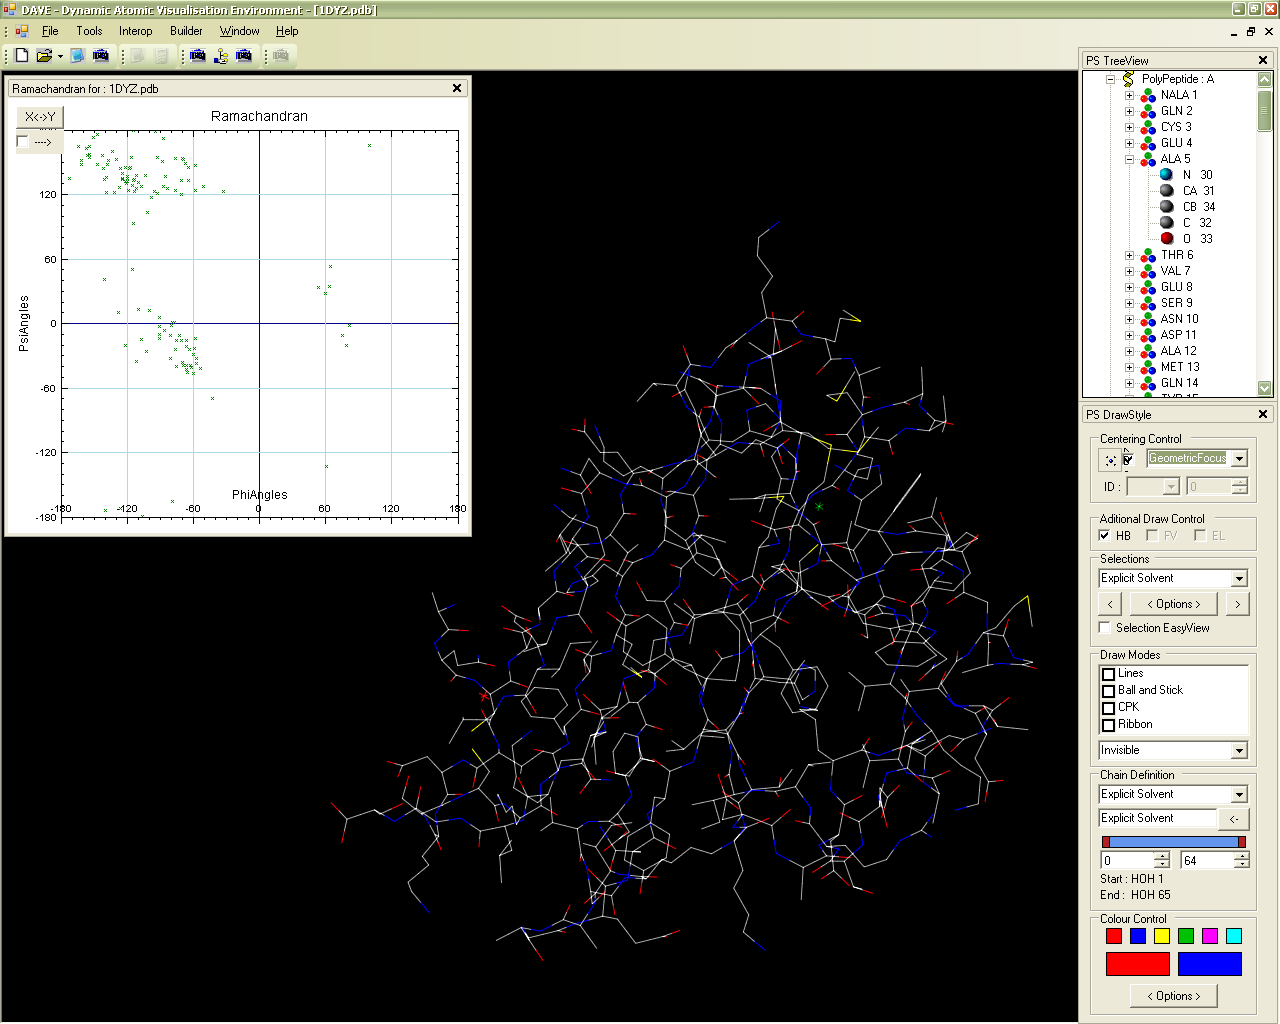
\includegraphics[width=0.75\textwidth]{03-Software/dave/main.png}
\caption{\dave: shown with a protein view, a tree-view representation of the atoms present, graphical options and dynamic Ramachandran plot.}
\label{fig:software:davemain}
\end{center}
\end{figure}

\begin{figure}[p]
\begin{center}
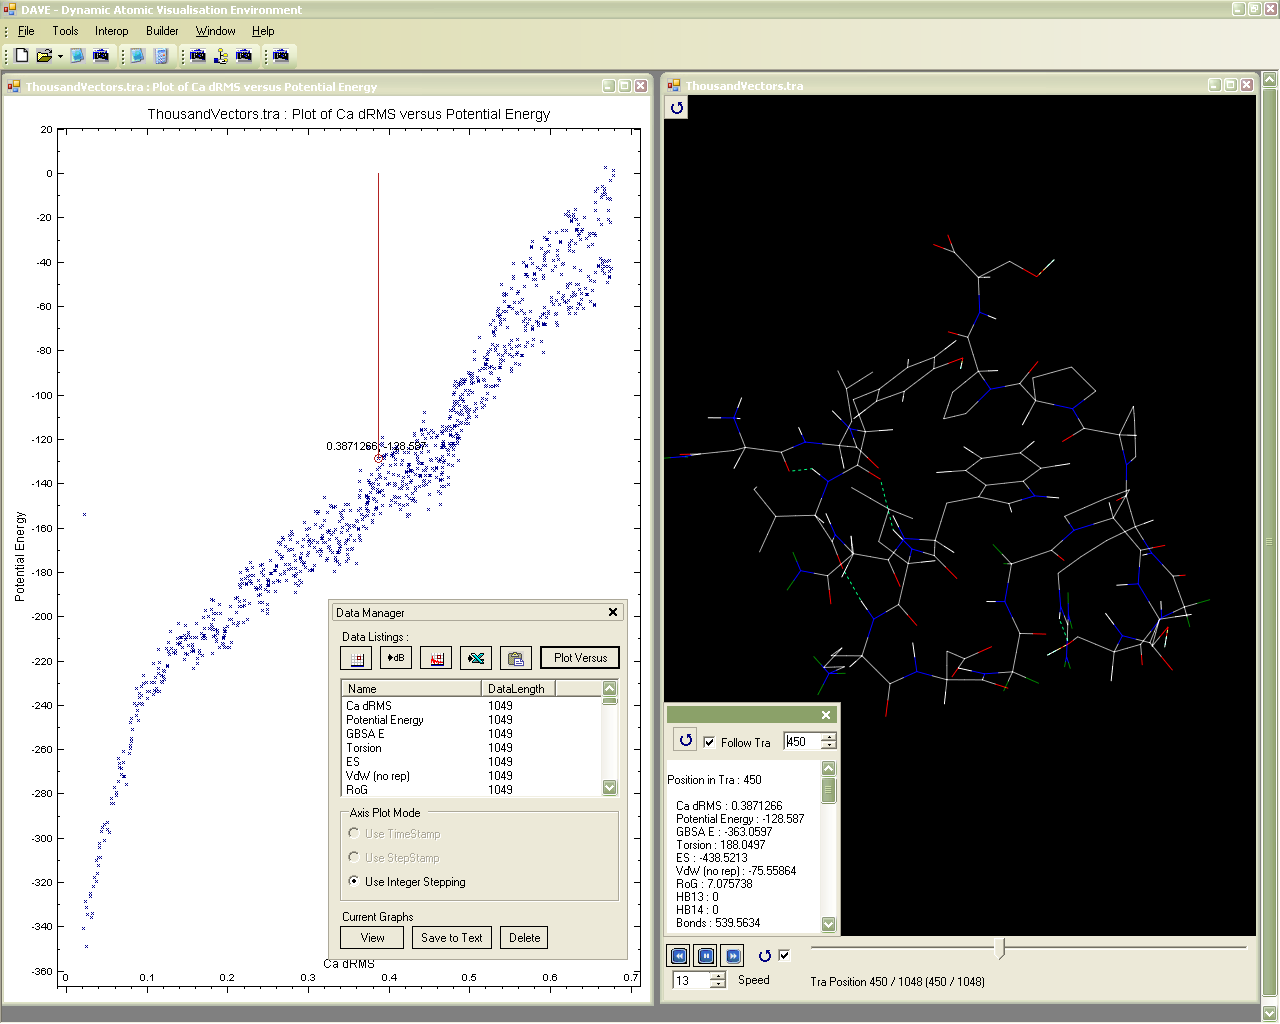
\includegraphics[width=0.75\textwidth]{03-Software/dave/graphing.png}
\caption{\dave: shown with a simulation of the TrpCage mini-protein and associated data. This includes a plot of energy vs. \ca-RMSD and a dynamic per-frame data box.}
\label{fig:software:davegraph}
\end{center}
\end{figure}

\subsection{Concluding Remarks}

The current implementation of the \uobf\ includes 55,497 lines of \CS\ source code, including 30,973 for the Core assembly, 18,169 lines dedicated to user interface components and just 5,961 lines dedicated to analysis tools. The relatively small amount of code dedicated to analysis stems form the concise interface that the framework core provides to its functionality. This is also represented by the fact that \dave\ and \pdbdb, although exhibiting significant functionality, are written in only 3,225 and 956 lines of code respectively.
It is clear that many other new scientific applications could potentially benefit from this shared base-code.
\clearpage
\section{Conclusions}

For this work two complementary frameworks have been developed to aid both molecular simulation algorithm development and data mining, totalling over 126,000 lines of code. This software, whilst still in rigourous development, is beginning to mature and as such is of real potential benefit to the research community. Both frameworks are soon to be made publicly available with a free academic licence. In terms of simulation, it is hoped that by combining a vast wealth of functionality into a single framework with a powerful front-end, the historical practise of having multiple small applications with separately maintained and overlapping functionality will be stemmed.  




